
\documentclass[preprint,12pt]{elsarticle}

\usepackage{graphicx,times,amsmath,amsfonts,subfig,array,multirow,url,algorithm,algorithmic,float,cleveref,pgfplots,bm}
\usepackage[flushleft]{threeparttable}
\usepackage{empheq}
\usepackage{booktabs}
\usepackage{tabularx}
\pgfplotsset{compat=1.12}
\usepackage{xifthen}
\usetikzlibrary{calc, positioning}
\usepackage{color,soulutf8}
\usepackage{tikz-cd,adjustbox,afterpage}

\definecolor{lightyellow}{cmyk}{0,0,0.5,0}
\sethlcolor{lightyellow}

\newcommand{\highlight}[1]{%
  \colorbox{yellow!50}{$\displaystyle#1$}}

\journal{Information Sciences}

\begin{document}

\begin{frontmatter}

\title{Multi-Target Support Vector Regression Via Correlation Regressor Chains}

\author[a]{Gabriella Melki}\author[a]{Alberto Cano}\author[a]{Vojislav Kecman}\author[b,c]{Sebasti\'an Ventura}

\address[a]{Department of Computer Science, Virginia Commonwealth University, USA}
\address[b]{Department of Computer Science and Numerical Analysis, University of Cordoba, Spain}
\address[c]{Department of Computer Science, King Abdulaziz University, Saudi Arabia Kingdom}

\begin{abstract}
Multi-target regression is a challenging task that consists of creating predictive models for problems with multiple continuous target outputs. Despite the increasing attention on multi-label classification, there are fewer studies concerning multi-target (MT) regression. The current leading MT models are based on ensembles of regressor chains, where random, differently ordered chains of the target variables are created and used to build separate regression models, using the previous target predictions in the chain. \hl{The challenges of building MT models stem from trying to capture and exploit possible correlations among the target variables during training.}
This paper presents three multi-target support vector regression models. The first involves building independent, single-target Support Vector Regression (SVR) models for each output variable. The second builds an ensemble of random chains using the first method as a base model. \hl{The third calculates the targets' correlations and forms a maximum correlation chain, which is used to build a single chained support vector regression model, improving the models' prediction performance while reducing the computational complexity.} The experimental study evaluates and compares the performance of the three approaches with \hl{seven other state-of-the-art multi-target regressors on $24$ multi-target datasets}. The experimental results are then analyzed using non-parametric statistical tests. The results show that the maximum correlation SVR approach improves the performance of using ensembles of random chains.
\end{abstract}

\begin{keyword}
Multi-target regression \sep multi-output regression \sep regressor chains \sep support vector regressor.
\end{keyword}

\end{frontmatter}

\section{Introduction}
In supervised learning, \textit{single-target} (ST) models are trained to predict the value of a single, categorical or numeric, target attribute of a given example. In some cases, more than one target, or output, can be associated with a single sample input. These situations are handled by a generalization of ST learning, which involves predicting these multiple outputs concurrently, and is known as multi-target (MT) learning~\cite{Aho2012,Borchani2015}. Specifically, MT learning includes \textit{multi-target regression} (MTR), which addresses the prediction of continuous targets, \textit{multi-label classification}~\cite{Zhang20141819} which focuses on binary targets, and \textit{multi-dimensional classification} which describes the prediction of discrete targets~\cite{Borchani2015,Read20141720}. 

Multi-target prediction has the capacity to generate models representing a wide variety of real-world applications, ranging from natural language processing~\cite{Jeong2009} to bioinformatics~\cite{Lui2010}. Other application areas include ecology~\cite{Aho2012}, gene function prediction~\cite{Kocev2015}, predicting the quality of vegetation~\cite{Hadavandi2015-2,Kocev2010}, stock price index forecasting~\cite{Xiong2014}, and operations research~\cite{Borchani2015,Hadavandi2015}. 

Constructing models for these types of real-world problems presents many challenges, such as missing data, (due to targets not being observed or recorded), and noisy data (due to instrument, experimental or human error)\hl{, and the curse of high dimensionality}. \hl{Along with these challenges, the most difficult task is identifying relationships between the input data and its corresponding output value. In the context of multi-target modeling, multiple outputs must now be trained against, which inherently adds computational complexity. The targets may or may not be correlated, and the corresponding model must accommodate for both scenarios.} However, a characteristic of the MT datasets used in these applications and elsewhere, is that they are generated by a single system, \hl{most likely} indicating that the nature of the outputs captured has some structure~\cite{Hadavandi2015}. Even though modeling the multi-variate nature and complex relationships between the target variables is challenging~\cite{Borchani2015}, they are more accurately represented by an MT model.% rather than an ST model. 

Several base-line methods have been proposed for solving multi-target tasks such as \hl{Multi-Objective Random Forests~{\cite{Kocev2010}}, Boosted Neural Networks~{\cite{Hadavandi2015-2}}, Ensembles of Trees~{\cite{Kocev2013}}, and many others. Support Vector Machines are a popular set of linear and non-linear supervised machine learning algorithms with a strong theoretical basis on Vapnik-Chervonenkis theory~{\cite{Vapnik1995}}. It has previously been shown that they outperform most algorithms in terms of performance, scalability, and the ability to efficiently deal with outliers}~\cite{Drucker1997,Kecman}. \hl{Input space dimensionality does not have an adverse effect on the model training time, and furthermore, the final model produced is sparse, allowing for quick predictions.}

\hl{There are two main approaches for using such base-line methods in the context of MT learning.} The first being \textit{problem transformation} methods, or \textit{local} methods, in which the multi-target problem is transformed into multiple single-target problems, each solved separately using \hl{classical methods, as described above.} The second being \textit{algorithm adaptation} methods, or \textit{global}, or \textit{big-bang} methods, that adapt existing single-target methods to predict all the target variables simultaneously~\cite{Borchani2015,Kocev2015}.
Using \textit{problem transformation} algorithms for a domain of \textit{t} target variables, \textit{t} predictive models must be constructed, each predicting a single-target variable~\cite{Kocev2015}. Prediction for an unseen sample would be obtained by running each of the \textit{t} single-target models and concatenating their results. Conversely, when using \textit{algorithm adaptation} algorithms for the same domain of \textit{t} target variables, only one model would need to be constructed which would output all \textit{t} predictions.

\hl{Literature shows} that \textit{algorithm adaptation} methods perform better than \textit{problem transformation} methods~\cite{Kocev2015,Spyromitros2014}. The most valuable advantage of using multi-target techniques is that, not only are the relationships between the sample variables and the targets exploited, but the relationships between the targets amongst themselves are as well~\cite{Baxter1997,Caruana1997}. Single-target techniques, on the other hand, eliminate any possibility of learning from the possible relationships between the target variables because a single, independent model is trained for each target separately~\cite{BenDavic2003}. Another advantage of MT techniques is model interpretability~\cite{Aho2012,Xiong2014}. A single multi-target model is highly more interpretable than a series of single-target models \hl{because it not only exploits the relationship between the data and targets, but also the targets amongst themselves.} Not only is a single MT model more interpretable, but it could also be considerably more computationally efficient to train, rather than training multiple single-target models individually~\cite{Appice2014}. 

This paper proposes three novel approaches to solving multi-target regression problems. The objective of this research topic is to investigate \hl{the performance changes when} building a regression model using \hl{two distinct \textit{algorithm adaptation} chaining methods versus} building independent single-target models for each target variable \hl{using a novel framework.} \hl{The main contributions presented in this paper include:}

\begin{itemize}
\item \hl{Evaluating the performance of a Support Vector Regressor (SVR) as a multi-target to single-target \textit{problem transformation} method to determine whether it outperforms current state-of-the-art ST algorithms. We analyze its performance as a base-line model for MT chaining methods due to the fact that ST methods do not account for any correlation among the target variables.}
\newpage

\item \hl{Building an MT ensemble of randomly chained SVR models (SVRRC), an \textit{algorithm adaptation} approach, inspired by the state-of-the-art chaining classification method, Ensemble of Random Chains Corrected (ERCC) {\cite{Xiong2014}}, to investigate the effects and advantages of exploiting correlations among target variables during model training, in the context of regression problems. The main issues to be investigated with this approach are the \textit{randomness} of the created chains because they might not capture of correlations between the targets, as well as the time taken to build all the regressors in the ensemble.}

\item \hl{Proposing an MT \textit{algorithm adaptation} model of SVRs that builds a unique chain, capturing the maximum correlation among target outputs, named SVR Correlation Chains (SVRCC). The advantages of using this \textit{maximum correlation chain} approach include exploiting the correlations among the targets which leads to an improvement in model prediction performance, and a reduction in computational complexity because a single SVR-chain model is trained, rather than building an ensemble of 10 base regressors.}
\end{itemize}

The experimental study evaluates and compares the performance of the three approaches, together with  \hl{7} other state-of-the-art multi-target regressors, on a set of \hl{24} datasets with varied input size, \hl{dimensionality}, and output targets. The results of the experiments are analyzed using non-parametric statistical analysis, namely the \hl{Bonferroni-Dunn, Holm, and  Wilcoxon} tests~\cite{Garcia20102044}. These post-hoc tests involve multiple comparisons among the algorithms, where they show significant differences in \hl{model} performances across all datasets. The statistical analysis of the experiments presented in this paper shows the increase in performance of the support vector regressors, specifically, the maximum correlation chain, SVRCC.

The paper is structured as follows. Section~\ref{sec:background} reviews related works on multi-target regression. Section~\ref{sec:proposal} presents the three multi-target support vector regression approaches. Section~\ref{sec:experiments} presents the experimental environment and study. Section~\ref{sec:results} \hl{shows} the results and statistical analysis. Finally, Section~\ref{sec:conclusions} shows the main conclusions of this work.
\newpage
\section{Background}\label{sec:background}
This section defines first the notation that will be used in the paper \hl{and formally} describes the multi-target regression problem along with the relevant state-of-the-art algorithms. 

\begin{table*}[b!]
\renewcommand{\arraystretch}{1.2}
\centering
\caption{Notation}
\begin{threeparttable}
\resizebox{\textwidth}{!}{\begin{tabular}{ll}
\toprule
Definition & Notation\\ 
\midrule
Number of Samples & $\mathcal{N}$ \\
Number of Input Attributes & $d$ \\
Input Space & $\bm{X} = \{\bm X_1, \ldots, \bm X_i, \ldots, \bm X_d\} \in \mathbb{R}^{\mathcal{N} \times d},\,1\leq i \leq d$ \\
Input Instance & $\bm{x}^{(l)} = (x_1^{(l)}, \ldots, x_d^{(l)}) \in \bm{X},\, 1 \leq l \leq\mathcal{N}$ \\
Number of Dataset Targets/Outputs & $m$ \\
Target Space & $\bm{Y} = \{\bm Y_1, \ldots, \bm Y_j, \ldots, \bm Y_m\} \in \mathbb{R}^{\mathcal{N} \times m},\, 1 \leq j \leq m$ \\
Predicted Target Space & $\bm{\hat{Y}} = \{\bm{\hat{Y_1}}, \ldots, \bm{\hat{Y_j}}, \ldots, \bm{\hat{Y}_m}\} \in \mathbb{R}^{\mathcal{N} \times m},\, 1 \leq j \leq m$ \\
\vspace{1.5pt}
Target Instance & $\bm y^{(l)} = (y_1^{(l)}, \ldots, y_m^{(l)}) \in \bm{Y},\,1 \leq l \leq\mathcal{N}$ \\
\hline
\noalign{\vskip 0.04in}
Full Multi-Target (MT) Training Dataset & $\mathcal{D} = \{(x_1^{(1)},y_1^{(1)}), \ldots, (x_d^{(\mathcal N)},y_m^{(\mathcal N)})\}$ \\
Single-Target (ST) Dataset with $j^{th}$ Target & $\mathcal{D}_j = \{(x_1^{(1)},y_j^{(1)}), \ldots, (x_d^{(\mathcal N)},y_j^{(\mathcal N)})\} \in \mathcal{D},\, 1 \leq j \leq m$\\
Number of Cross-Validation (CV) Sets & $k$ \\
ST Test Dataset with $j^{th}$ Target, $i^{th}$ CV Fold & $\mathcal{D}_j^{(i)} = \{(x_1^{(i)},y_j^{(i)}), \ldots, (x_d^{(i)},y_j^{(i)}) \in \mathcal{D}_j,\, i \in \{1,\ldots,\mathcal{N}\}$ \\
ST Training Dataset with $j^{th}$ Target, Excluding the $i^{th}$ CV Fold & $\mathcal{D}_j^{(k-i)} = \mathcal{D}_j \setminus \mathcal{D}_j^{(i)}$ \\
MT Regression Model & $h : \bm{X} \times \bm{Y}$ \\
ST Regression Model & $h_j : \bm{X} \times \bm{Y}_j,\, 1 \leq j \leq m$ \\
Unknown Sample & $\bm{x}^{(\mathcal N^\prime)} = \{\bm {x}^{(\mathcal N+1)}, \ldots, \bm {x}^{\mathcal (N^\prime)}\}$ \\
Predicted Values for Unknown Sample & $\bm{y}^{(\mathcal N^\prime)} = \{\bm{y}^{(\mathcal N+1)}, \ldots, \bm {y}^{(\mathcal N^\prime)}\}$\\
\bottomrule
\end{tabular}}
\end{threeparttable}
\label{tab:Notation}
\bigskip
\end{table*}

\subsection{Notation}\label{subsec:notation}
Let $\mathcal{D}$ be a training dataset of $\mathcal{N}$ instances \hl{and their continuous outputs}. Let $\bm{X} \in \mathcal{D}$ be a matrix consisting of $d$ input variables and $\mathcal{N}$ samples, sometimes called input space, having a domain of $\bm{X} \in \mathbb{R}^{\mathcal{N} \times d}$. Let $\bm{Y} \in \mathcal{D}$ be a matrix consisting of $m$ target variables for the $\mathcal{N}$ input samples, sometimes called output space, having a domain of $\bm{Y} \in \mathbb{R}^{\mathcal{N} \times m}$. For each sample $(\bm x^{(l)},\bm y^{(l)}) \in \mathcal{D}$, $\bm{x}^{(l)} = (x_1^{(l)}, \ldots, x_d^{(l)})$ and $\bm y^{(l)} = (y_1^{(l)}, \ldots, y_m^{(l)})$ are the input and output vectors respectively, where $l \in \{1, \ldots, \mathcal{N}\}$. Using the training dataset $\mathcal{D} = \{(\bm x^{(1)},\bm y^{(1)}), \ldots, (\bm x^{(\mathcal{N})},\bm y^{(\mathcal{N})})\}$, the goal is to learn a multi-target regression model $h : \bm{X} \times \bm{Y}$, that assigns a vector $\bm{y}$ with $m$ target values, for each input instance $\bm{x}$. The model will then be used to predict the values of $\{\bm{y}^{(\mathcal{N}+1)}, \ldots, \bm{y}^{(\mathcal{N}^\prime)}\}$ for new unlabeled input vectors $\{\bm{x}^{(\mathcal{N}+1)}, \ldots, \bm{x}^{(\mathcal{N}^\prime)}\}$. Table~\ref{tab:Notation} summarizes the notation used in this paper.

\subsection{Multi-Target Regression Methods}\label{subsec:mtr}
In the context of \textit{problem transformation} for multi-target models, $m$ single-target models will be trained on the dataset $\mathcal{D}_j = \{(x_1^{(1)},y_j^{(1)}), \ldots, (x_d^{(N)},y_j^{(\mathcal{N})})\}$, where $j \in \{1, \ldots, m\}$. This way there are $m$ independent, single-target models, one model for each target variable. This is described as the baseline Single-Target (ST) model in~\cite{Spyromitros2014}. A generalized visualization of the \textit{problem transformation} method is shown in Table~\ref{tab:pt}. Many \textit{problem transformation} methods have been proposed to solve multi-target problems, which are detailed next.

\begin{table}[!t]
\renewcommand{\arraystretch}{1.6}
\centering
\caption{Transformation to $m$ Single-Target Datasets}
\begin{tabular}{ccc}
\hline
Dataset & Values & Output \\
\hline
$\mathcal{D}_1$ & $\{(x_1^{(1)},y_1^{(1)}), \ldots, (x_d^{(\mathcal{N})},y_1^{(\mathcal{N})})\}$ & $h_1 : \mathcal{D}_1 \rightarrow \mathbb{R}$ \\
$\mathcal{D}_2$ & $\{(x_1^{(1)},y_2^{(1)}), \ldots, (x_d^{(\mathcal{N})},y_2^{(\mathcal{N})})\}$ & $h_2 : \mathcal{D}_2 \rightarrow \mathbb{R}$ \\
$\vdots$ & $\vdots$ & $\vdots$ \\
$\mathcal{D}_j$ & $\{(x_1^{(1)},y_j^{(1)}), \ldots, (x_d^{(\mathcal{N})},y_j^{(\mathcal{N})})\}$ & $h_j : \mathcal{D}_j \rightarrow \mathbb{R}$ \\
$\vdots$ & $\vdots$ & $\vdots$ \\
$\mathcal{D}_m$ & $\{(x_1^{(1)},y_m^{(1)}), \ldots, (x_d^{(\mathcal{N})},y_m^{(\mathcal{N})})\}$ & $h_m : \mathcal{D}_m \rightarrow \mathbb{R}$ \\
\hline
\end{tabular}
\label{tab:pt}
\end{table}

\hl{Many authors have proposed using Support Vector Machines (SVM) for multi-target learning}~\cite{Borchani2015,Xiong2014,Xu2013}. \hl{SVMs have some similarities to various classification and regression problems, but research has shown that in terms of scalability, robustness against outliers, and their efficiency in learning form large and sparse datasets, they are a very useful machine learning tool that can be used in diverse real world applications}~\cite{Chen20152502,Kecman,Melki2016,Zhu2017292}.

\hl{Zhang et al.{~\cite{Zhang2012}} presented a multi-output support vector regression approach based on problem transformation. It builds a multi-output model that considers the correlations between all the targets using the vector virtualization method. Basically, it extends the original feature space and expresses the multi-output problem as an equivalent single-output problem, so that it can then be solved using the single-output least squares support vector regression machines (LS-SVR) algorithm. \textit{Xiong et. al.} presented a support vector regression method with a firefly heuristic in{~\cite{Xiong2014}}, in the context of interval forecasting of a stock price index. Originally proposed in{~\cite{msvr}}, the algorithm was then modified with a firefly heuristic, named FA-MSVR, to intelligently identify the appropriate SVR hyper-parameters. To produce attractive results using support vector machines, appropriate hyper-parameters must be selected. This is a crucial and computationally expensive step to ensure the SVR model is performing to the best of its capabilities{~\cite{Zhao2015160}}. The results obtained by \textit{Xiong et. al.} indicate that FA-MSVR proved to be a promising alternate method for time series forecasting, thus highlighting the importance of setting the SVR hyper-parameters.}

Moreover, other approaches based on Linear Target Combinations for MT Regression~\cite{Tsoumakas2014}, and Multi-Objective  \hl{Random Forests} (MORF) \cite{Kocev2007} have been proposed. Most commonly investigated issues for MT learning problems include dimensionality reduction for high-dimensional multi-labeled data. The curse of dimensionality is problematic due to the possible correlations between the data and the targets~\cite{Charte20141842,Ding20152521,He2011}. This multi-collinearity may cause the learning task to be more difficult and complex~\cite{Qian2015594}. To reduce the dimensionality of the data, without losing the possible relationships to the targets, careful feature selection could be performed, which is a difficult task as well~\cite{Lee201580,Li2016827}. Another issue would be processing large datasets quickly and feasibly (because of memory constraints), while providing insightful information~\cite{Borchani2015, 2016-INS-LAIM}.

The \hl{RC}, MTS, MTSC, ERC, and ERCC methods are introduced by \textit{Spyromitros et. al.} in~\cite{Spyromitros2014}. The idea behind these algorithms was to investigate whether advances in multi-label learning can be successfully used and implemented in a multi-target regression setting, as well as shedding light on modeling target dependencies. They first describe the \hl{RC, MTS,} and ERC models, which are  inspired by multi-label classification algorithms, and then introduce their corrected versions. These  methods involve two stages of learning, the first being building ST models and the second uses the knowledge gained by the first step to predict the target variables while using possible relationships the target variables might have with one another. 

The two stages of training in MTS involve firstly, training $m$ independent single-target models, like in ST. In the second step, a second set of $m$ meta models are learned for each target variable, $\bm{Y}_j,\, 1 \leq j \leq m$. These meta models are learned on a transformed dataset, where the input attributes space is expanded by adding the approximated target variables obtained in the first stage, excluding the $j^{th}$ target being predicted. Each $m$ meta model, $h_j^* : \bm{X} \times \mathbb{R}^{m-1} \rightarrow \mathbb{R}$, is learned by the modified dataset $\mathcal{D}_j^* = \{(x_1^{*(1)},y_j^{*(1)}), \ldots, (x_d^{*(\mathcal{N})},y_j^{*(\mathcal{N})})\}$, where $\bm x_j^{*(l)} = \{x_1^{(l)}, \ldots, x_d^{(l)}, \hat{y}_1^{(l)}, \ldots, \hat{y}_{j-1}^{(l)}, \hat{y}_{j+1}^{(l)}, \ldots, \hat{y}_m^{(l)}\},\, l \in \{1, \ldots, \mathcal{N}\}$ are the input vectors along with the $m-1$ predicted target variables, represented by $\hat{\bm y}$, obtained by the first step. To predict the output for a new input vector $\bm{x}^{(q)}$, the models trained in the first stage are applied and an output vector, $\hat{\bm{y}}^{(q)} = \{\hat{\bm{y}}_1^{(q)}, \ldots, \hat{\bm{y}}_m^{(q)}\} = \{h_1(\bm{x}^{(q)}), \ldots, h_m(\bm{x}^{(q)})\}$, is obtained. The second stage models are then applied on the transformed input vector $\bm x_j^{*(q)}$, as shown above, to produce a final output vector.

The ERC method is somewhat similar to the MTS method. In the training of a Regression Chain (RC) model, a random chain, or sequence, of the set of target variables is selected and for each target in the chain, models are built sequentially by using the output of the previous model as input for the next~\cite{Xioufis2016}. If the default, ordered chain is $C = \{\bm Y_1, \bm Y_2, \ldots, \bm Y_m\}$, the first model $h_1 : \bm X \rightarrow \mathbb{R}$ is trained for $\bm Y_1$, as in ST. For the subsequent models $h_{j,j>1}$, the dataset is transformed into $\mathcal{D}_j^* = \{(\bm x_j^{*(1)},y_j^{(1)}), \ldots, (\bm x_j^{*(\mathcal{N})},y_j^{(\mathcal{N})})\}$, where $\bm x_j^{*(l)} = \{x_1^{(l)}, \ldots, x_d^{(l)}, y_1^{(l)}, \ldots, y_{j-1}^{(l)}\}$ are the input vectors transformed by sequentially appending the true values of each of the previous targets in the chain. For a new input vector $\bm{x}^{(q)}$, the target values are unknown. So  once the models are trained, the unseen input vector $\bm{x}^{(q)}$ will be appended with the approximated target values, making the models dependent on the approximated values obtained in each step. One of the issues associated with this method is that, if a single random chain is used, the possible relationships between the targets at the head of the chain and the end of the chain are not exploited due to the algorithm's sequential nature. Also, prediction error in the earlier stages of the models will be propagated as the rest of the models are trained, which is why the Ensemble of Regressor Chains was proposed in ~\cite{Spyromitros2014}. Instead of a single chain, $k$ chains are created at random, and the final prediction values are obtained by taking the mean values of the $k$ predicted values for each target. 

In the methods described above, the estimated target variables (meta-variables) are used as input in the second stage of training. In both methods, the models are trained using these meta-variables that become noisy at prediction time, and thus the relationship between the meta-variables and target variable is muddied. Dividing the training set into sets, one for each stage, would not help this situation because both methods would be trained on training sets of decreasing size. Due to these issues, \textit{Spyromitros et. al.} proposed modifications, in \cite{Spyromitros2014}, to both methods that resembles $k$-fold cross-validation (CV) to be able to obtain unbiased estimates of the meta-variables. These methods are called Regression Chains Corrected (RCC) and Multi-Target Stacking Corrected (MTSC). 

The ERCC and MTSC procedures involve repeating the RCC and MTS procedures $k$ times, respectively, with $k$ randomly ordered chains for ERCC, and $k$ different modified training sets for MTSC. The algorithms were tested and compared using Bagging of $100$ regression trees as their base regression algorithm with ERC and ERCC ensemble size of $10$, and $10$-fold cross-validation. The corrected methods exhibited better performance than their original variants, as well as ST models. The ERCC algorithm had the best overall performance, as well as being statistically significantly more accurate of all the methods tested. These methods can be found and used through the open-source Java library, Mulan~\cite{mulan}; to replicate the results found in~\cite{Spyromitros2014}. 

The following section presents our approaches to solving the multi-target regression problem inspired by the techniques presented in~\cite{Spyromitros2014}. It will show that exploiting and making use of the possible correlations in the target variables produces better results than not. 

\section{Multi-target SVR proposal}\label{sec:proposal}

Three novel models have been implemented for the purposes of multi-target regression. The  \hl{base-line model is the \textit{problem transformation} method, named}  SVR, where $m$ single-target soft-margin non-linear support vector regressors (NL-SVR) are built for each target variable $\bm Y_j$. For NL-SVR, the regularized soft-margin loss function given in equation \eqref{eq:softsvropt} is minimized~\cite{Drucker1997,Kecman},

\begin{subequations}\label{eq:softsvropt}
\begin{equation}
\begin{aligned}
\underset{\bm{w},\xi,\xi^*}{\text{minimize}} & \ \ \ \ \frac{1}{2}||\bm{w}||^2 + C\sum_{l=1}^\mathcal{N}{\left(\xi^{(l)} + \xi^{*(l)} \right)}
\end{aligned}
\tag{\ref{eq:softsvropt}}
\end{equation}
\begin{empheq}[left={\text{subject to}\  }\empheqlbrace]{align}
y^{(l)}-\langle \bm{w},\phi\left(\bm{x}^{(l)}\right)\rangle \leq \epsilon + \xi^{(l)} \\
\langle \bm{w},\phi\left(\bm{x}^{(l)}\right)\rangle-y^{(l)} \leq \epsilon + \xi^{*(l)} \\
\xi^{(l)}, \xi^{*(l)} \geq 0 
\end{empheq}
\end{subequations}

where $\bm{w}$ represents the SVR weight vector, $\epsilon$ represents how precise the approximations are, $C > 0$ determines how to penalize deviations from $\epsilon$, $\phi(\cdot)$ represents a feature mapping function, $\xi^{(l)}$ and $\xi^{*(l)}$ are slack variables, and $y^{(l)}$ is the label corresponding to the input vector $\bm{x}^{(l)}$. For simplicity, the bias SVR term has been excluded. In our algorithm implementation, the dual of this formulation~\cite{Vapnik1995,Drucker1997} given by \eqref{eq:dualsvr} is solved,

\begin{subequations}\label{eq:dualsvr}
\begin{equation}
\begin{aligned}
\underset{\bm{\alpha},\bm{\alpha}^*}{\text{maximize}} & \ \ \ -\frac{1}{2}\sum_{l,k=1}^{\mathcal{N}}{\left(\bm{\alpha}^{(l)}-\bm{\alpha}^{*(l)}\right)\left(\bm{\alpha}^{(k)}-\bm{\alpha}^{*(k)}\right)}\mathcal{K}\left(\bm{x}^{(l)},\bm{x}^{(k)}\right)\\
{} & -\epsilon\sum_{l=1}^{\mathcal{N}}{\left(\bm{\alpha}^{(l)}+\bm{\alpha}^{*(l)}\right)} + \sum_{l=1}^{\mathcal{N}}{y^{(l)}\left(\bm{\alpha}^{(l)}-\bm{\alpha}^{*(l)}\right)} 
\end{aligned}
\tag{\ref{eq:dualsvr}}
\end{equation}
\begin{eqnarray}
\text{subject to} & \sum_{l=1}^{\mathcal{N}}{\left(\bm{\alpha}^{(l)}-\bm{\alpha}^{*(l)}\right)=0},\ \ \bm{\alpha}^{(l)},\bm{\alpha}^{*(l)} \in \left[0,C\right]
\end{eqnarray}
\end{subequations}

where the $\boldsymbol{\alpha}$ and $\boldsymbol{\alpha^*}$ vectors correspond to the SVR dual variables and \\$\mathcal{K}\left(\bm{x}^{(l)},\bm{x}^{(k)}\right) = \phi(\bm{x}^{(l)})^\prime * \phi(\bm{x}^{(k)})$ is an $\left({\mathcal{N}} \times {\mathcal{N}}\right)$ Gaussian kernel matrix which is dependent on the $\gamma$ parameter for its broadness. Using the SVR optimization problem described, the multi-target problem is solved by transforming it into $m$ single-target problems, as shown in Algorithm~\ref{alg:SVR} \hl{and Figure}~\ref{diag:SVR}. This algorithm will output $m$ single-target models, $h_j,\,\forall j = 1,\ldots,m$, for a given dataset $\mathcal{D}$. It first splits the dataset into $m$ separate ones, each with a single-target variable $\bm Y_j$, and then builds a distinct SVR model for each of the datasets. \hl{For predicting the output values for a new and unseen instance, each of the $m$ models would have to be run on the same sample, and then aggregate their independent outputs.}


%%%%%%%%%% SVR ALG %%%%%%%%%%%%%%%
\begin{figure}
\caption{\hl{SVR Flow Diagram}}
\small
\label{diag:SVR}
\centering
\begin{minipage}{0.9\textwidth}
\[\begin{tikzcd}[column sep = small, row sep = small]
& & \mathcal{D}_1 :  [\bm X][\bm Y_1]  \arrow[rr]  & & h_1 :  \mathcal{D}_1 \rightarrow \bm{\hat{Y_1}}\\
& & \mathcal{D}_2 :  [\bm X][\bm Y_2]  \arrow[rr] & & h_2 :  \mathcal{D}_2 \rightarrow \bm{\hat{Y_2}} \\        
\mathcal{D} :  [\bm X][\bm Y]  \arrow[uurr, bend left=45] \arrow[urr, bend left] \arrow[drr, bend right]  		& & \vdots \\
& & \mathcal{D}_m :  [\bm X][\bm Y_m] \arrow[rr] & & h_m :  \mathcal{D}_m \rightarrow \bm{\hat{Y}_m}
\end{tikzcd}\]
{\footnotesize Firstly, the SVR method separates the MT dataset into $m$ ST datasets, $\mathcal{D}_1, \mathcal{D}_2, \ldots, \mathcal{D}_m$. It then independently trains models, $h_1, h_2, \ldots, h_m$, for each ST dataset.\par}
\end{minipage}
\begin{algorithm}[H]
\caption{\hl{MT Support Vector Regression (SVR)}}
\small
\centering
\label{alg:SVR} 
\begin{algorithmic}[1]
\renewcommand{\algorithmicrequire}{\textbf{Input:}}
\renewcommand{\algorithmicensure}{\textbf{Output:}}
\REQUIRE Training dataset $\mathcal{D}$, number of cross-validation folds $k$
\ENSURE  ST models $h_j, j = 1,\ldots,m$
\FOR {$j = 1$ to $m$}
\STATE $\mathcal{D}_j = \{(x_1^{(1)},y_j^{(1)}), \ldots, (x_d^{(\mathcal N)},y_j^{(\mathcal N)})\}$
\\ \textit{Create the CV training $\mathcal{D}^{(k-i)}$ and test $\mathcal{D}^{(i)}$ sets}
\FOR {$i=1$ to $k$}
\STATE $\mathcal{D}_j^{(k-i)} = \{(x_1^{(k-i)},y_j^{(k-i)}), \ldots, (x_d^{(k-i)},y_j^{(k-i)})\}$ 
\STATE $\mathcal{D}_j^{(i)} = \{(x_1^{(i)},y_j^{(i)}), \ldots, (x_d^{(i)},y_j^{(i)})\}$ 
\\ \textit{Train the $j^{th}$ model on the training set $\mathcal{D}^{(k-i)}$}
\STATE $h_j^{(k-i)} : \mathcal{D}_j^{(k-i)} \rightarrow \mathbb{R}$
\\ \textit{Test the $j^{th}$ model on the test set $\mathcal{D}^{(i)}$}
\STATE $\hat{\bm Y}_j^{(i)} = h_j^{(k-i)}(\bm X^{(i)})$
\ENDFOR
\\ \textit{Calculate and store aRRMSE error for the $j^{th}$ model}
\ENDFOR
\RETURN $h_j, j=1,\ldots,m$ 
\end{algorithmic} 
\end{algorithm}
\end{figure}

\hl{There are many advantages of using an SVM as a base-line model. Firstly, the optimization problem defining it contains a regularization parameter, which prevents model overfitting to the training dataset{~\cite{Boyd}}. Secondly, the optimization problem is convex, indicating a unique global minimum, which can be found efficiently. Furthermore, it also allows for use of the kernel trick which allows for more flexibility and knowledge in model training as well as a final sparse model, based only on the number of support vectors{~\cite{Kecman}}.}

Building $m$ ST models was a good base-line model, but as mentioned previously, it does not use any of the possible correlations between the target attributes during training. If these correlations are not exploited, it could retract from the model's potential performance. Therefore, we also proposed to construct a series of random chains and create an ensemble model, as done in~\cite{Spyromitros2014}, but using our base-line SVR method, named SVR Random Chains (SVRRC). For SVRRC, ensembles of at most $10$ random chains are built, with length $m$, of different and distinct permutations of the target variable indices. For each chain, we train $m$ chained models using the targets true values. \hl{An illustration of this process is shown in Figure}~\ref{fig:svrrc}. Due to the computational complexity of building $m!$ distinct chains and training $\left(m!\right) \times m$ models, the number of ensembles and chains are limited to a maximum of $10$~\cite{Spyromitros2014}. However, if the number of target variables is less than $3$, i.e. $m! \leq 10$, we construct all $m!$ random chains. For each of the random chains, the model is trained by predicting the first target variable in the chain. Next, the first target's true value, $\bm Y_j$, is appended to the end of the training set as such, $\mathcal{D}_{j+1}^* = \{\bm X_{j+1}^*, \bm Y_j\}$, where $\bm X_{j+1}^*$ is the appended training set, ${\bm X_{j+1}^* = \{x_1^{(l)},\ldots,x_d^{(l)},y_1^{(l)},\ldots,y_j^{(l)}\},l=\{1,\ldots,\mathcal N\}}$. 

The chaining process is repeated for all the target indices in the chains. When chaining target values, there are two main options: using the predicted value as input for the following target, or using the true value of the target variable as input of the subsequent targets. The main problem with the former approach is that errors are propagated \hl{throughout the training process. As each estimated, predicted value gets appended to the train set, additional noise now exists in the input space when training for the next target.} \hl{However, the latter approach,} minimizes error propagation,  \hl{resulting in a more accurate model}. Our approach  employs chaining of the true values\hl{, rather than appending the targets estimation produced while training}. Given the ensemble of SVRs, the predicted values for a given instance are calculated by taking the mean of the multiple models generated using different random chains. For predicting unseen inputs that have no target values, the predicted value at each step of the chain $\hat{y_j}^{(l)}$ is appended to the input as shown in Algorithm~\ref{alg:SVRCP}. For SVRRC described in Algorithm~\ref{alg:SVRRC}, at most $10$ models will be built (one for each chain $RC$, $RC_c = \{RC_c^{(1)}, \ldots, RC_c^{(m)}\}, \, c \leq 10 \,$), each iterating and training $m$ chained models. \hl{For each of the models in the chain, we use $10$-fold cross-validation to ensure the hyper-parameters chosen best describe the data.}

%%%%%%%%%%%%%%% SVRRC %%%%%%%%%%%%%%%%%%%%%%%

\begin{figure}[tpb]
\centering
\caption{\hl{SVRRC Flow Diagram}}
\small
\label{fig:svrrc}
\begin{minipage}{0.9\textwidth}
\adjustbox{scale=0.88}{%
\begin{tikzcd}[column sep = small, row sep = small]
& \mathcal{D} :  [\bm X][\bm Y_1 \bm Y_2 \bm Y_3] \arrow[dl] \arrow[d] \arrow[drr] & & \\
\left[1,2,3\right] \arrow[d] & \left[1,3,2\right] \arrow[d] & \hdots & \left[3,2,1\right] \arrow[d] \\
h_1 :  [\bm X] \rightarrow \bm{\hat{Y_1}} \arrow[d] & h_1 :  [\bm X] \rightarrow \bm{\hat{Y_1}} \arrow[d] & \hdots & h_1 :  [\bm X] \arrow[d] \\
h_2 :  [\bm X \bm{Y_1} ] \rightarrow \bm{\hat{Y_2}} \arrow[d] & h_2 :  [\bm X \bm{Y_1} ] \rightarrow \bm{\hat{Y_3}} \arrow[d] & \hdots & h_2 :  [\bm X \bm{Y_3} ] \rightarrow \bm{\hat{Y_2}} \arrow[d] \\
h_3 :  [\bm X \bm{Y_1Y_2} ] \rightarrow \bm{\hat{Y_3}} & h_3 :  [\bm X \bm{Y_1Y_3} ] \rightarrow \bm{\hat{Y_2}} & \hdots & h_3 :  [\bm X \bm{Y_3Y_2} ] \rightarrow \bm{\hat{Y_1}}
\end{tikzcd}}

{\footnotesize This figure illustrates how the SVRRC algorithm trains a dataset with $3$ target variables. It first builds the $6$ random chains of the target's indices ($3$ examples are shown). It then constructs a chained model by proceeding recursively over the chain, building a model, and appending the current target to the input space to predict the next target in the chain. \par}
\end{minipage}
\begin{algorithm}[H]
\caption{\hl{MT SVR with Random-Chains (SVRRC)}}
\small
\label{alg:SVRRC} 
\begin{algorithmic}[1]
\renewcommand{\algorithmicrequire}{\textbf{Input:}}
\renewcommand{\algorithmicensure}{\textbf{Output:}}
\REQUIRE Training dataset $\mathcal{D}$, number of cross-validation folds $k$
\ENSURE  $c$ chained models $h_j, j = \{1,\ldots,m\}, c \leq 10$
\STATE $RC_c^{(m)}$, \textit{    Create at most $10$ distinct random chains of size $m$}
\STATE $\mathcal{D}_1^* = \{(x_1^{(1)},y_1^{(1)}),\ldots,(x_d^{(\mathcal N)},y_1^{(\mathcal N)})\}$
\FOR {$j=1$ to $m$}
\STATE $h_j : \mathcal{D}_j^* \rightarrow \mathbb{R}$
\IF {$j < m$}
\STATE $\mathcal{D}_{j+1}^* \leftarrow \emptyset$
\FOR {$i=1$ to $k$}
\STATE $h_j^{(i)} : \mathcal{D}_j^{(k-i)} \rightarrow \mathbb{R}$
\\ \textit{Test the model on the test set $D_j^{*(i)}$}
\FOR {$\bm x^{*(i)} \in \mathcal{D}_j^{*(i)}$}
\STATE $\hat{y}_j^{(i)} = h_j^{(i)}(\bm x^{*(i)})$
\\ \textit{Append $\bm x^{*(i)}$ with the true value $y_j^{(i)}$, and add it to set $\mathcal{D}_{j+1}^*$}
\STATE $\mathcal{D}_{j+1}^* = \mathcal{D}_{j+1}^* \cup [\bm x^{*(i)},y_j^{(i)}]$
\ENDFOR
\ENDFOR
\ENDIF
\ENDFOR
\RETURN $h_j, j=1,\ldots,m$ 
\end{algorithmic} 
\end{algorithm}
\end{figure}


\begin{figure}[tpb]
\caption{\hl{SVRCC Flow Diagram}}
\label{fig:svrcc}
\centering
\begin{minipage}{0.9\textwidth}
\adjustbox{scale=0.975}{%
\begin{tikzcd}
\mathcal{D} :  [\bm X][\bm Y_1 \bm Y_2 \bm Y_3] \arrow{rr}{\textit{generate maximum correlation chain}}[swap]{\frac{\mathbf{E}\left[(Y_i - \mu_i)(Y_j - \mu_j)\right]}{\sqrt{\mathbf{E}\left[(Y_i - \mu_i)(Y_i - \mu_i)\right]\mathbf{E}\left[(Y_j - \mu_j)(Y_j - \mu_j)\right]}}} 
&  \arrow[d, phantom, ""{coordinate, name=Z}]
& \left[1,2,3\right]  \arrow[dll, rounded corners, to path={ -- ([xshift=1ex]\tikztostart.east)
|- ([yshift=-2.5ex]Z) [near end]\tikztonodes
-| ([xshift=-1ex]\tikztotarget.west)
-- (\tikztotarget)}] \\
h_1 :  [\bm X] \rightarrow \bm{\hat{Y_1}} \arrow[r]
& h_2 :  [\bm X \bm{Y_1} ] \rightarrow \bm{\hat{Y_2}} \arrow[r]
& h_3 :  [\bm X \bm{Y_1Y_2} ] \rightarrow \bm{\hat{Y_3}} 
\end{tikzcd}}

{\footnotesize This figure shows how the SVRCC algorithm trains a sample dataset with $3$ target variables. It first finds the direction of maximum correlation among the targets and uses that order as the only chain. It then constructs the chained model as done in SVRRC. \par}
\end{minipage}

\begin{algorithm}[H]
\caption{\hl{MT SVR with Max-Correlation Chain (SVRCC)}}
\small
\label{alg:SVRCC} 
\begin{algorithmic}[1]
\renewcommand{\algorithmicrequire}{\textbf{Input:}}
\renewcommand{\algorithmicensure}{\textbf{Output:}}
\REQUIRE Training dataset $\mathcal{D}$, number of cross-validation folds $k$
\ENSURE  Chained model $h_j, j = \{1,\ldots,m\}$
\STATE $correlation_{\left(m \times m\right)} = corrcoef(\bm Y)$
\STATE $sums_m = sum\left(correlation\left(l,j\right)\right), l=1,\ldots,m$
\\ \textit{Create the maximum correlation chain $c$ of size $m$}
\STATE $c_m = sort\left(sums_m,\textbf{decreasing}\right)$
\STATE $\mathcal{D}_{c_1}^* = \{(x_1^{(1)},y_{c_1}^{(1)}),\ldots,(x_d^{(\mathcal N)},y_{c_1}^{(\mathcal N)})\}$
\FOR {$j=1$ to $m$}
\STATE $h_{c_j} : \mathcal{D}_{c_j}^* \rightarrow \mathbb{R}$
\IF {$j < m$}
\STATE $\mathcal{D}_{c_{j+1}}^* \leftarrow \emptyset$
\\ \textit{Split $\mathcal{D}_{c_j}^*$ into $k$ disjoint parts $\mathcal{D}_{c_j}^{*(i)}, \, i=1,\ldots,k$ for training and testing}
\FOR {$i=1$ to $k$}
\STATE $h_{c_j}^{(i)} : \mathcal{D}_{c_j}^{*(k-i)} \rightarrow \mathbb{R}$
\\ \textit{Test the model on the test set $\mathcal{D}_{c_j}^{*(i)}$}
\FOR {$\bm x^{*(i)} \in \mathcal{D}_{c_j}^{*(i)}$}
\STATE $\hat{y}_{c_j}^i = h_{c_j}^{(i)}(\bm x^{*(i)})$
\\ \textit{Append $\bm x^{*(i)}$ with the true value $y_{c_j}^{(i)}$, and add it to set $\mathcal{D}_{c_{(j+1)}}^*$}
\STATE $\mathcal{D}_{c_{(j+1)}}^* = \mathcal{D}_{c_{(j+1)}}^* \cup [\bm x^{*(i)},y_{c_j}^{(i)}]$
\ENDFOR
\ENDFOR
\ENDIF
\ENDFOR
\RETURN $h_j, j = \{1,\ldots,m\}$
\end{algorithmic} 
\end{algorithm}
\end{figure}

When the number of output variables increases, the number of possible chains increases factorially. Therefore, there is no guarantee that the random chains generated will truly reflect the relationships among the target variables. Moreover, building an ensemble of regressors is computationally expensive. Finding a heuristic that allows the identification of a single, most appropriate chain, which fully reflects the output variable interrelations would improve the computational complexity of training the ensemble. Our third proposal builds a single chain based on the maximization of the correlations among the target variables. By calculating the correlation of the target variables and imposing that on the order of the chain, we ensure that each appended target provides some additional knowledge on the training of the next. With SVRRC, there is no proof or reasoning behind the generation of these chains, and since the number of random chains generated is limited to $10$, there is no way of ensuring that the $10$ chains fully represent the targets' dependencies. Therefore, calculating and using the correlations of the targets would break this uncertainty, as done in the SVR Correlation Chain (SVRCC) method, shown in Algorithm~\ref{alg:SVRCC} \hl{and Figure~{\ref{fig:svrcc}}. The computational complexity and hardware constraints (memory size) of constructing the targets' $(m \times m)$ correlation matrix are only dependent on the number of targets. This eliminates the additional complexity of creating and aggregating at most $m$ randomly chained models.} To calculate the correlation coefficients of the targets, we first construct the targets' co-variance matrix, $\sum_{i,j} = cov(Y_i,Y_j) = \mathbf{E}\left[(Y_i - \mu_i)(Y_j - \mu_j)\right]$, where $\mu_i = \mathbf{E}(Y_i)$, and $\mathbf{E}(Y_i)$ is the expected value of $Y_i$, $\forall i,j \in \{1,\ldots,m\}$. The correlation coefficient matrix is then calculated as follows, $\rho_Y = corrcoef(Y) = \frac{cov(Y_i,Y_j)}{\sqrt{cov(Y_i,Y_i)cov(Y_j,Y_j)}}$, $\forall i,j \in \{1,\ldots,m\}$. The correlation coefficient matrix will describe the linear relationship among the target variables and then they can be sorted in decreasing order, creating the maximum correlation chain. Having a single chain reduces the computational complexity, while providing a competitive model. For an unknown sample, the prediction method  \hl{follows the same procedure} as Algorithm~\ref{alg:SVRCP}\hl{, where the predicted value $\hat{y_j}^{(l)}$ is appended to the input}. 

\begin{algorithm}[H]
\caption{\hl{SVR Chained Prediction}}
\small
\label{alg:SVRCP} 
\begin{algorithmic}[1]
\renewcommand{\algorithmicrequire}{\textbf{Input:}}
\renewcommand{\algorithmicensure}{\textbf{Output:}}
\REQUIRE Unknown sample $\bm x^{(q)}$, chained model ${h_j, j=\{1...m\}}$
\ENSURE  Output vector $\hat{\bm y}^{(q)}$ of size $m$
\\ \textit{Initialize the output vector}
\STATE $\hat{\bm y}^{(q)} = \textbf{0}$
\\ \textit{Initialize the input space for the first target}
\STATE $\mathcal{D}_1^* = \bm x^{(q)}$
\FOR {$j=1$ to $m$}
\STATE $\bm x^* \in \mathcal{D}_j^*$
\STATE $\hat{y}_j^{(q)} = h_j(\bm x^*)$
\STATE $\mathcal{D}_{j+1}^* = \mathcal{D}_j^* \cup [\bm x^*, \hat{y}_j^{(q)}]$
\ENDFOR
\\ \textit{Create ST transformation of $\mathcal{D}$ with $1^{st}$ index in chain $c$}
\RETURN $\hat{\bm y}^{(q)}$ 
\end{algorithmic} 
\end{algorithm}

\section{Experiments}\label{sec:experiments}
This section presents the experimental comparison of the three models proposed, along with  \hl{seven} others from state-of-the-art. \hl{It introduces the datasets, algorithms, performance measures, and statistical analysis.} 

\subsection{Datasets}\label{subsec:data}
This section presents a description of the datasets used in the experiments. Although there are many interesting applications of multi-target regression, there are \hl{few} publicly available datasets to use. The datasets used in the experimental study were collected from the Mulan website~\cite{mulan}, as well as the UCI Machine Learning Repository~\cite{Lichman:2013}. Information on \hl{the $24$ datasets} used is summarized in Table~\ref{tab:datasets}, where the number of samples, attributes (dimensionality), and targets are shown. Note that the datasets used in this experiment are the same datasets used in~\cite{Spyromitros2014} to properly perform our model comparisons, as well as  additional datasets \hl{to ensure thorough investigation}. 
%
%\begin{itemize}
%\item \textbf{Electrical Discharge Machining} The EDM dataset's purpose is to optimize the machining time by approximating the behavior of a human operator who controls the values of two variables, gap control and flow control. 
%
%\item \hl{\textbf{Enb} The Energy and Buildings dataset is used to analyze the effect of eight input variables on the heating and cooling load of residential buildings}~\cite{Tsanas2012}.
%
%\item \hl{\textbf{Jura} The Jura dataset is used to analyze 7 geochemical characteristics of land and rock at 356 different locations.}~\cite{Goo1997}.
%
%\item \hl{\textbf{Osales} The Online Product Sales dataset is used to identify patterns in the online sales of a consumer product based on product feature data}~\cite{Kaggle2012}.
%
%\item \hl{\textbf{Scpf} The See Click Predict Fix dataset is used to predict which \textit{311} issues are most important to citizens}~\cite{Kaggle2013}.
%
%\item \hl{\textbf{Slump} The Slump dataset is used to predict 3 characteristics of the slump flow of high performance concrete}~\cite{Yeh2007}.
%
%\item \textbf{Solar Flare 1 \& Solar Flare 2} The Solar Flare dataset~\cite{mulan} is used for predicting how often 3 types of solar flare are observed in 24 hours. The three types of solar flare - common, moderate, and severe. 
%\item \textbf{Water Quality} The Water Quality dataset~\cite{mulan} is used for approximating 14 target attributes that represent chemicals found in Slovenian rivers. 16 input attributes describing the biology of the river, the chemistry and physical water quality, are used to predict the target variables.
%\item \textbf{OES97 \& OES10} The Occupational Employment Survey datasets were compiled during the years 1997 (OES97) and 2010 (OES10) ~\cite{mulan}. There are 16 targets that are randomly selected from a set of employment categories.
%\item \textbf{ATP1d \& ATP7d} The Airline Ticket Price datasets~\cite{mulan} are used to predict airline ticket prices. The 411 input variables include details about the different flights and the 6 targets are the minimum prices observed over the next 7 days for 6 airline preferences. 
%\item \hl{\textbf{Andro} The Andromeda dataset contains data produced by the Andromeda Analyzer; a device that gathers water quality data in the Thermaikos Gulf of Thessaloniki, Greece~{\cite{Hatzikos2008}.}}
%\item \textbf{Wisconsin Cancer} Each sample represents follow-up data for one breast cancer patient, who is exhibiting invasive breast cancer, and no evidence of metastases at the time of diagnosis. This dataset can be used to predict whether the cancer is recurrent, and the time in which it might recur. 
%\item \textbf{Stock} This dataset includes daily stock prices from January $1988$ through October $1991$ for $10$ aerospace companies.
%\item \textbf{California Housing} This dataset includes information on block groups of individuals in California, from the $1990$ Census. It contains $20,640$ samples with $7$ continuous attributes, which are used to predict the $2$ target variables, median house value and the median income.
%\item \textbf{Puma8NH \& Puma32H} The Puma8H and Puma32H datasets are synthetically generated from a simulation of the dynamics of a Unimation Puma 560 robot arm~\cite{Lichman:2013}, used to predict the angular acceleration of one robot arm link. The inputs, 8 for Puma8H and 32 for Puma32H, include angular positions, velocities, and torques of the robot arm.
%\item \textbf{Friedman} This is an artificial dataset where $25$ attributes of each of the samples are generated independently from a uniform distribution over $[0,1]$. To measure the effects of non-related attributes, additional attributes are added to the datasets, which are independent from the output. 
%\item \textbf{Polymer} The Polymer Test Plant dataset contains $10$ input variables representing measurements of controlled variables, such as temperatures, feed rates, etc., in a polymer processing plant. The $4$ target variables are the measurements of the output of that plant.
%\item \textbf{M5SPEC \& MP5SPEC \& MP6SPEC} These datasets consist of $80$ corn samples measured on $3$ different NIR spectrometers, M5, MP5, and MP6.
%\end{itemize}

\begin{table*}[!b]
\centering
\scriptsize
\caption{\hl{Multi-Target Regression datasets}}
\begin{tabular}{lccc}
\hline
Dataset & Samples $(\mathcal N)$ & Attributes $(d)$ & Targets $(m)$\\
\hline
EDM & 145 & 16 & 2\\
\hl{Enb} & \hl{768} & \hl{8} & \hl{2} \\
\hl{Jura} & \hl{359} & \hl{11} & \hl{7} \\
\hl{Osales} & \hl{639} & \hl{413} & \hl{12} \\
\hl{Scpf} & \hl{1137} & \hl{23} & \hl{3} \\
\hl{Slump} & \hl{103} & \hl{7} & \hl{3} \\
Solar Flare 1 & 323 & 10 & 3\\
Solar Flare 2 & 1,066 & 10 & 3\\
Water Quality & 1,060 & 16 & 14\\
OES97 & 323 & 263 & 16\\
OES10 & 403 & 298 & 16\\
ATP1d & 201 & 411 & 6\\
ATP7d & 188 & 411 & 6\\
\hl{Andro} & \hl{49} & \hl{30} & \hl{6} \\
Wisconsin Cancer & 198 & 34 & 2\\
Stock & 950 & 10 & 3\\
California Housing & 20,640 & 7 & 2\\
Puma8NH & 8,192 & 8 & 3\\
Puma32H & 8,192 & 32 & 6\\
Friedman & 500 & 25 & 6\\
Polymer & 41 & 10 & 4\\
M5SPEC & 80 & 700 & 3\\
MP5SPEC & 80 & 700 & 3\\
MP6SPEC & 80 & 700 & 3\\
\hline
\end{tabular}
\label{tab:datasets}
\end{table*}

\subsection{Algorithms}\label{subsec:algorithmsres}
This section presents the algorithms that we compare our proposals' performances to; namely \hl{\textit{RC, ST, MTS, MTSC, ERC, ERCC,}} and \textit{MORF} which has been used in the experimental study conducted in~\cite{Spyromitros2014}. Our contributions are compared to these algorithms because they have shown considerable performance in training multi-target models. The have also made their framework readily available for reproducing their results, allowing proper comparisons to be made with their methods. Moreover, note that all three SVR algorithms are implemented within the general framework of Mulan's MTRegressor\footnote{http://mulan.sourceforge.net}~\cite{mulan}, which was built on top of Weka\footnote{http://www.cs.waikato.ac.nz/ml/weka}~\cite{weka}, and we also used LIBSVM's Epsilon-SVR~\cite{CC01a} implementation of Support Vector Regressors as the base SVR model.

\hl{In order to train a model that accurately describes a dataset and is not over-fit, experimenting with different model hyper-parameters is required. In the case of SVMs, specifically the SVM regression task, these parameters are the penalty parameter $C$, the Gaussian kernel parameter $\gamma$, and the error or tube parameter $\epsilon$. We experimented with a range of parameters given in equations~{\eqref{eq:paramC}} to~{\eqref{eq:paramE}}, referred to as~{\eqref{eq:hyperparam}}, to ensure the final model is best representative of the dataset the model is being trained on. We have compared the models trained on the different hyper-parameters using $k$-fold cross-validation, which ensures that the models' performances are accurately assessed, and the model built is not biased towards the full dataset. This is a crucial step in evaluating the generalizability and efficiency of the trained models on an independent dataset.}
\begin{subequations}
\label{eq:hyperparam}
\begin{align}
\highlight{C \in}  & \highlight{\{1, 10, 100\}} \label{eq:paramC}\\
\highlight{\gamma \in}  & \highlight{\{1^{-9}, 1^{-7}, 1^{-5}, 1^{-3}, 1^{-1}, 1, 5, 10\}} \label{eq:paramG}\\
\highlight{\epsilon \in}  & \highlight{\{0.01, 0.1, 0.2\}} \label{eq:paramE}
\end{align}
\end{subequations}

To ensure having a controlled environment when conducting our performance comparisons, the experimental environment for running the competing algorithms was the same as what was done in~\cite{Spyromitros2014}. This includes the following. The ST base-line model used was Bagging~\cite{Breiman1996} of 100 regression trees~\cite{Wu2015430}. The MTSC and ERCC methods are run using $10$-fold cross-validation, and the ensemble size for the ERC and ERCC methods was set to $10$. The ensemble size of 100 trees was used for MORF, and the rest of its parameters were set as recommended by~\cite{Kocev2013}.

The main preprocessing step used for the experiments was normalization. The input variables were scaled to have a mean value of $0$ and standard deviation of $1$. To ensure that each sample is used when building the final model, we used sampling without replacement when creating our training and testing sets. \hl{The preprocessed and final datasets used in the experiments, along with the code for the algorithms presented in this paper, can be publicly found here\footnote{http://people.vcu.edu/$\sim$acano/MTR-SVRCC}.}

\subsection{Performance Evaluation}\label{subsec:perfeval}
The performance metric\hl{s} used to analyze our contributions' performances  \hl{are} shown in Equation\hl{s}~\ref{eqn:aCC} to~\ref{eqn:arrmse}. For unseen or test datasets of size $\mathcal N_{test}$, the performances are evaluated by taking the  \hl{the run time (seconds) each algorithm takes to build a classifier, as well as the following metrics}~\cite{Borchani2015,Friedman2010}\hl{, where the upwards arrow $\uparrow$ indicates maximizing the metric and the downwards arrow $\downarrow$ indicates minimizing the metric.}

\begin{itemize}
\item \hl{The average correlation coefficient (aCC $\uparrow$):}
\begin{eqnarray}
\highlight{\frac{1}{m} \sum_{j = 1}^m \frac{\sum_{l = 1}^{\mathcal N_{test}} (y_j^{(l)} - \bar{y}_j)(\hat{y}_j^{(l)} - \bar{\hat{y}}_j)}{\sqrt{\sum_{l = 1}^{\mathcal N_{test}} (y_j^{(l)} - \bar{y}_j)^2 \sum_{l = 1}^{\mathcal N_{test}} (\hat{y}_j^{(l)} - \bar{\hat{y}}_j)^2}}}
\label{eqn:aCC}
\end{eqnarray}

\item \hl{The mean squared error (MSE $\downarrow$):}
\begin{eqnarray}
\highlight{\frac{1}{m} \sum_{j = 1}^m \frac{1}{\mathcal N_{test}} \sum_{l = 1}^{\mathcal N_{test}} (y_j^{(l)} - \hat{y}^{(l)}_j)^2}
\label{eqn:MSE}
\end{eqnarray}

\item \hl{The average root mean squared error (aRMSE $\downarrow$):}
\begin{eqnarray}
\highlight{\frac{1}{m} \sum_{j = 1}^m \sqrt{\frac{\sum_{l = 1}^{\mathcal N_{test}} (y_j^{(l)} - \hat{y}^{(l)}_j)^2}{\mathcal N_{test}}}}
\label{eqn:armse}
\end{eqnarray}

\item \hl{The average relative root mean squared error (aRRMSE $\downarrow$):}
\begin{eqnarray}
\highlight{\frac{1}{m} \sum_{j = 1}^m \sqrt{\frac{\sum_{l = 1}^{\mathcal N_{test}} (y_j^{(l)} - \hat{y}_j^{(l)})^2}{\sum_{l = 1}^{\mathcal N_{test}} (y_j^{(l)} - \bar{y}_j)^2}}}
\label{eqn:arrmse}
\end{eqnarray}
\end{itemize}

\hl{The predicted output is represented by $\hat{\textbf{y}}$, the average of the predicted output is $\bar{\hat{\textbf{y}}}$, and the average of the true output target variable is $\bar{\textbf{y}}$.} The test dataset is the hold-out set during cross validation. This ensures our model is evaluated on data that it has not been trained on, and thus unbiased towards the training datasets. \hl{It also contributes to the generalizability and robustness of the model.}

\section{Results \& Statistical Analysis}\label{sec:results}
\hl{This section presents the results obtained by each metric of the $10$ algorithms (columns) on $24$ multi-target datasets (rows), along with the averaged results, average rank according to Friedman~{\cite{Garcia20102044}}, and statistical analysis. Tables~{\ref{tab:accresults}},~{\ref{tab:mseresults}},~{\ref{tab:armseresults}},~{\ref{tab:arrmseresults}}, and~{\ref{tab:timeresults}} show the results of the metrics, described in Section~{\ref{subsec:perfeval}}, of our algorithm implementations compared with those of \textit{RC, MORF, ST, MTS, MTSC, ERC,} and \textit{ERCC}. Each subsection discusses a single metric along with the statistical analysis of the results. The best metric value obtained on each dataset is typeset in bold.}

\hl{In order to compare the performances of the multiple models, non-parametric statistical tests are used to validate the experiments results obtained}~\cite{Derrac2011,Garcia20102044}\hl{. To determine whether significant differences exist among the performance and results of the algorithms, the Iman-Davenport non-parametric test is run~{\cite{Garcia2008}}. It is applied to rank the algorithms over the datasets used, according to the Friedman test, where the best performing algorithm is given rank 1, the next best given rank 2, and so on. The average ranks are presented in the last row of the results tables, and the lowest rank value is typeset in bold. Having the rank values helps in determining the best performing algorithm across all datasets and metrics.}

\hl{The Iman-Davenport test indicates statistically significant differences, then the Bonferroni-Dunn post-hoc test~{\cite{Dunn1961}} is used to find these differences that occur between the algorithms. The test assumes that the two classifiers performances are significantly different if their average ranks differ by at least some critical value~{\cite{Garcia2009}}. Below each result table, a diagram highlighting the critical distance (in gray) between each algorithm is shown.  }

\hl{The Wilcoxon, Nemenyi, and Holm~{\cite{Wilcoxon1945}} tests were run for each of the result metrics to compute multiple pairwise comparisons among the proposed algorithms and the state-of-the-art methods. The tests determine whether significant differences between pairs of algorithms exist. Tables~{\ref{tab:statacc}},~{\ref{tab:statmse}},~{\ref{tab:statarmse}},~{\ref{tab:statarrmse}}, and~{\ref{tab:stattime}} show the sum of ranks $R^+$ and $R^-$ of the Wilcoxon rank-sum test, and the $p$-values for the $3$ tests, which show the statistical confidence rather than using a fixed $\alpha$ value.}

\subsection{Average Correlation Coefficient}\label{subsec:acc}
\hl{Table~{\ref{tab:accresults}} shows that our proposed methods perform the best on $15$ out of the $24$ datasets. Specifically, the maximum correlation chain method, SVRCC, performs the best on $11$, which is better than the total number of datasets the state-of-the-art methods performed better at ($9$). The Iman-Davenport statistic, distributed according to the F-distribution with 9 and 207 degrees of freedom is $6.72$, with a $p$-value of $1.9E^{-8}$ which is significantly less than $0.01$, implying a statistical confidence larger than $99\%$. Therefore, we can conclude that there exist statistically significant differences between the aCC results of the algorithms.}

\hl{Figure~{\ref{fig:BonfDunnACC}} shows the mean rank values of each algorithm along with the critical difference value, $2.4236$, for $\alpha = 0.05$. The algorithms that are to the right of the critical difference rectangle are the ones with significantly different results. Therefore, the $6$ out of $10$ algorithms beyond the critical difference perform significantly worse than our control algorithm, SVRCC.}

\hl{Table~{\ref{tab:statacc}} provides complementary analysis of the results. According to the Wilcoxon test, SVRCC is shown to have significantly better performance over all algorithms with $p$-value $< 0.05$. The Nemenyi and Holm tests show that SVRCC performs significantly better than $6$ out of the $9$ algorithms with $p$-value $\leq 5.6E^{-3}$ and $\leq 1.7E^{-2}$, respectively. The exact confidence for algorithm SVRCC against all others is $0.95$.}

\afterpage{%
\begin{table*}[thp!]
\renewcommand{\arraystretch}{1.2}
\centering
\caption{\hl{Average Correlation Coefficient (aCC) Results \& Algorithm Rank}}
\small
\begin{threeparttable}
\resizebox{0.9\textwidth}{!}{\begin{tabular}{lccccccccccc}
\toprule
Datasets &MORF &ST &MTS &MTSC &RC &ERC &ERCC &SVR &SVRRC &SVRCC \\
\midrule
Slump &0.6965 &0.7062 &0.7163 &0.6977 &0.6956 &0.6977 &0.7023 &0.7245 &0.7339 &\textbf{0.7457} &  \\
Polymer &0.7305 &0.7336 &0.7371 &0.7228 &0.7015 &0.7029 &0.7222 &0.7634 &0.7857 &\textbf{0.7905} &  \\
Andro &\textbf{0.7349} &0.6454 &0.6793 &0.6581 &0.6915 &0.6806 &0.6653 &0.6880 &0.6951 &0.7056 &  \\
EDM &\textbf{0.6722} &0.6352 &0.6412 &0.6354 &0.6355 &0.6379 &0.6354 &0.6484 &0.6565 &0.6567 &  \\
Solar Flare 1 &0.1083 &0.1258 &0.1034 &0.1193 &\textbf{0.1492} &0.1387 &0.1292 &0.1066 &0.0857 &0.1152 &  \\
Jura &0.7854 &0.7907 &0.7880 &0.7882 &0.7877 &0.7884 &0.7897 &0.7789 &0.7921 &\textbf{0.7983} &  \\
Enb &0.9828 &0.9832 &0.9822 &0.9829 &0.9813 &0.9823 &0.9837 &0.9858 &0.9867 &\textbf{0.9868} &  \\
Solar Flare 2 &0.2357 &0.2295 &0.2375 &0.2343 &0.2302 &0.2351 &\textbf{0.2432} &0.1470 &0.1648 &0.1656 &  \\
Wisconsin Cancer &0.3362 &0.3587 &\textbf{0.3652} &0.3588 &0.3628 &0.3609 &0.3590 &0.3187 &0.3208 &0.3373 &  \\
California Housing &0.7705 &0.7720 &0.7149 &0.7451 &0.7007 &0.7844 &\textbf{0.8065} &0.7847 &0.7949 &0.8007 &  \\
Stock &0.9785 &0.9747 &0.9755 &0.9752 &0.9753 &0.9757 &0.9763 &0.9825 &\textbf{0.9829} &0.9822 &  \\
SCPF &0.5827 &0.5508 &0.5503 &0.5477 &0.5569 &0.5656 &0.5515 &0.5891 &\textbf{0.5975} &0.5946 &  \\
Puma8NH &0.5424 &0.4828 &0.4942 &0.4205 &0.4677 &0.4656 &0.4650 &\textbf{0.6041} &0.5975 &0.6038 &  \\
Friedman &0.1507 &0.1609 &0.1548 &0.1667 &0.1558 &0.1608 &0.1632 &0.1710 &0.1748 &\textbf{0.1752} &  \\
Puma32H &0.3085 &0.2934 &0.2890 &0.2504 &0.2754 &0.2870 &0.2797 &0.3358 &0.3351 &\textbf{0.3385} &  \\
Water Quality &\textbf{0.4303} &0.4063 &0.4019 &0.4051 &0.3992 &0.4052 &0.4147 &0.3545 &0.3828 &0.3857 &  \\
M5SPEC &0.8161 &0.8346 &0.8134 &0.8228 &0.8333 &0.8340 &0.8308 &0.9451 &0.9452 &\textbf{0.9472} &  \\
MP5SPEC &0.8315 &0.8536 &0.8244 &0.8535 &0.8524 &0.8526 &0.8542 &0.9560 &0.9602 &\textbf{0.9633} &  \\
MP6SPEC &0.8317 &0.8531 &0.8231 &0.8531 &0.8507 &0.8515 &0.8541 &0.9444 &0.9500 &\textbf{0.9528} &  \\
ATP7d &0.8260 &0.8408 &0.8422 &\textbf{0.8474} &0.8273 &0.8351 &0.8464 &0.8305 &0.8407 &0.8400 &  \\
OES97 &0.7829 &0.7995 &0.7990 &0.8001 &0.7986 &0.7990 &0.7999 &0.8116 &0.8134 &\textbf{0.8137} &  \\
Osales &0.7186 &0.6912 &0.7104 &0.7076 &0.6357 &0.7136 &\textbf{0.7193} &0.6511 &0.6433 &0.6677 &  \\
ATP1d &0.8961 &0.9066 &0.9051 &0.9075 &0.9048 &0.9081 &0.9071 &0.9092 &\textbf{0.9130} &0.9100 &  \\
OES10 &0.8708 &0.8808 &0.8805 &0.8806 &0.8804 &0.8804 &0.8809 &0.8911 &0.8924 &\textbf{0.8963} &  \\
\hline
Average &0.6508 &0.6462 &0.6429 &0.6409 &0.6396 &0.6476 &0.6492 &0.6634 &0.6685 &\textbf{0.6739} &  \\
Ranks &6.4167 &5.8958 &6.6042 &6.4792 &7.5208 &5.8958 &4.8542 &4.7917 &3.7083 &\textbf{2.8333} &  \\
\bottomrule
\end{tabular}}
\end{threeparttable}
\label{tab:accresults}
\vspace{-2.5em}
\end{table*}
\begin{figure}[h!]
\centering
\small
\resizebox{0.8\textwidth}{!}{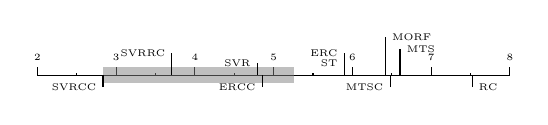
\begin{tikzpicture}
 %axis
 \draw (2,0) -- (8,0);
 \foreach \x in {2,3,4,5,6,7,8} {
  \draw (\x, 0) -- ++(0,.1) node [above,scale=0.7] {\tiny \x};
  \ifthenelse{\x < 8}{\draw (\x+.5, 0) -- ++(0,.03);}{}
 }
 % coordinates
 \coordinate (c0) at (2.8333,0);
 \coordinate (c1) at (3.7083,0);
 \coordinate (c2) at (4.7917,0);
 \coordinate (c3) at (4.8542,0);
 \coordinate (c4) at (5.8958,0);
 \coordinate (c5) at (7.5208,0);
 \coordinate (c6) at (6.4792,0);
 \coordinate (c7) at (6.6042,0);
 \coordinate (c8) at (5.8958,0);
 \coordinate (c9) at (6.4167,0);

 % labels
 \node (l0) at (c0) [below left=.025cm and 0cm, align=right, scale=0.7] {\tiny SVRCC};
 \node (l1) at (c1) [above left=.15cm and 0cm, align=right, scale=0.7] {\tiny SVRRC};
 \node (l2) at (c2) [above left=.025cm and 0cm, align=right, scale=0.7] {\tiny SVR};
 \node (l3) at (c3) [below left=.025cm and 0cm, align=left, scale=0.7] {\tiny ERCC};
 \node (l4) at (c4) [above left=.15cm and 0cm, align=right, scale=0.7] {\tiny ERC};
 \node (l5) at (c5) [below right=.025cm and 0cm, align=left, scale=0.7] {\tiny RC};
 \node (l6) at (c6) [below left=.025cm and 0cm, align=right, scale=0.7] {\tiny MTSC};
 \node (l7) at (c7) [above right=.2cm and 0cm, align=left, scale=0.7] {\tiny MTS};
 \node (l8) at (c8) [above left=.025cm and 0cm, align=right, scale=0.7] {\tiny ST};
 \node (l9) at (c9) [above right=.35cm and 0cm, align=right, scale=0.7] {\tiny MORF};

 % CD = 1.4845
 \fill[fill=gray,fill opacity=0.5] (2.8333,-0.1) rectangle (5.2569,0.1);
 
 % connectors
 \foreach \x in {0,...,9} {
  \draw (l\x) -| (c\x);
 };
\end{tikzpicture}}
\caption{\hl{Bonferroni-Dunn test for aCC}}
\label{fig:BonfDunnACC}
\end{figure}
\vspace{-1.6em}
\begin{table}[H]
\centering
\caption{\hl{Wilcoxon, Nemenyi, and Holm tests for aCC}}\label{tab:statacc}
\scriptsize
\begin{threeparttable}
\begin{tabularx}{0.6\textwidth}{p{1cm}p{1cm}p{1cm}p{1cm}p{1cm}p{0.9cm}}
\toprule
SVRCC vs. & Wilcoxon $R^{+}$ & Wilcoxon $R^{-}$ & Wilcoxon $p$-value & Nemenyi $p$-value & Holm $p$-value \\ 
\midrule 
MORF & 224.0 & 76.0 & $3.4E^{-2}$ & $4.1E^{-5}$& $8.3E^{-3}$ \\
ST & 239.0 & 61.0 & $9.6E^{-3}$ & $4.6E^{-4}$ & $1.3E^{-2}$ \\ 
MTS & 242.0 & 58.0 & $7.2E^{-3}$ & $1.6E^{-5}$ & $6.3E^{-3}$ \\ 
MTSC & 238.0 & 62.0 & $1.1E^{-2}$ & $3.0E^{-5}$ & $7.1E^{-3}$ \\ 
RC & 250.0 & 50.0 & $3.1E^{-3}$ & 0.0000 & $5.6E^{-3}$ \\
ERC & 229.0 & 71.0 & $2.3E^{-2}$ & $4.6E^{-4}$ & $1.0E^{-2}$ \\ 
ERCC & 221.0 & 79.0 & $4.3E^{-2}$ & $2.1E^{-2}$ & $1.7E^{-2}$ \\ 
SVR & 297.0 & 3.00 & $6.0E^{-7}$ & $2.5E^{-2}$ & $2.5E^{-2}$ \\ 
SVRRC & 266.5 & 33.5 & $4.0E^{-4}$ & $3.2E^{-1}$ & $5.0E^{-2}$ \\ 
\bottomrule
\end{tabularx}
\begin{tablenotes}
\item Post Hoc (Friedman) comparison for $\alpha = 0.05$
\end{tablenotes}
\end{threeparttable}
\end{table}}

\subsection{Mean Square Error}\label{subsec:mse}
\hl{Table~{\ref{tab:mseresults}} shows that our proposed methods perform the best on $15$ out of the $24$ datasets. In this case, SVRCC also performs the best on $11$ versus the $9$ that the state-of-the-art methods performed better at. The Iman-Davenport statistic, distributed according to the F-distribution with $9$ and $207$ degrees of freedom is $6.57$, with a $p$-value of $3.1E^{-8}$, implying statistically significant differences among the MSE results.}

\hl{Figure~{\ref{fig:BonfDunnMSE}} shows the mean rank values of each algorithm along with the critical difference value, $2.4236$, for $\alpha = 0.05$. According to the critical difference bar, there are $6$ out of $10$ algorithms beyond that perform significantly worse than our control algorithm, SVRCC.}

\hl{According to the Wilcoxon test, shown in Table~{\ref{tab:statmse}}, SVRCC is shown to have significantly better performance over all algorithms with $p$-value $< 0.05$. The Nemenyi and Holm tests show that SVRCC performs significantly better than $6$ out of the $9$ algorithms with $p$-values $\leq 5.6E^{-3}$ and $\leq 1.7E^{-2}$ respectively, and has an exact confidence of $0.95$ against all others.}

\afterpage{%
\begin{table*}[t!]
\renewcommand{\arraystretch}{1.2}
\centering
\small
\caption{\hl{Mean Square Error (MSE) Results \& Algorithm Rank}}
\begin{threeparttable}
\resizebox{0.9\textwidth}{!}{\begin{tabular}{lccccccccccc}
\toprule
Datasets &MORF &ST &MTS &MTSC &RC &ERC &ERCC &SVR &SVRRC &SVRCC \\
\midrule
Slump &1.4388 &1.4161 &1.3667 &1.4414 &1.4602 &1.4727 &1.4183 &1.2991 &1.1726 &\textbf{1.1614} &  \\
Polymer &1.6718 &1.8120 &1.5446 &1.6726 &1.8259 &1.9999 &1.6873 &1.1874 &1.1068 &\textbf{1.0796} &  \\
Andro &1.4930 &2.1467 &1.4714 &1.7525 &2.2603 &2.0812 &1.8707 &1.5406 &1.2847 &\textbf{1.2187} &  \\
EDM &\textbf{0.8342} &0.9373 &0.9352 &0.9418 &0.9389 &0.9326 &0.9393 &0.9092 &0.8650 &0.8817 &  \\
Solar Flare 1 &3.3458 &3.1196 &3.1193 &3.0524 &3.0357 &3.0381 &3.0594 &\textbf{2.9912} &3.0176 &3.0129 &  \\
Jura &1.0973 &1.0595 &1.0732 &1.0695 &1.0744 &1.0694 &1.0632 &1.1167 &1.0435 &\textbf{1.0315} &  \\
Enb &0.0381 &0.0361 &0.0407 &0.0377 &0.0452 &0.0403 &0.0343 &0.0255 &0.0216 &\textbf{0.0214} &  \\
Solar Flare 2 &2.9619 &2.8532 &\textbf{2.7732} &2.8282 &2.8510 &2.8273 &2.8110 &2.9518 &2.9204 &2.8713 &  \\
Wisconsin Cancer &1.7666 &1.7155 &1.7156 &1.7256 &\textbf{1.7119} &1.7146 &1.7195 &1.8171 &1.7915 &1.7692 &  \\
California Housing &0.8665 &0.8221 &0.9642 &0.8673 &1.0125 &0.8952 &0.7513 &0.7477 &0.6987 &\textbf{0.6726} &  \\
Stock &0.0841 &0.1039 &0.0990 &0.1008 &0.0998 &0.0987 &0.0949 &0.0578 &0.0596 &\textbf{0.0554} &  \\
SCPF &\textbf{2.2244} &2.3173 &2.3661 &2.3517 &2.3923 &2.3025 &2.3295 &2.2960 &2.2510 &2.3179 &  \\
Puma8NH &1.9678 &2.1133 &2.0989 &2.2024 &2.1413 &2.1473 &2.1467 &\textbf{1.8242} &1.8728 &1.8299 &  \\
Friedman &5.4573 &5.3357 &5.3478 &5.3260 &5.3482 &5.3253 &5.3210 &5.3038 &5.2942 &\textbf{5.2812} &  \\
Puma32H &5.3419 &\textbf{4.9499} &4.9627 &5.0405 &4.9905 &4.9662 &4.9805 &5.2711 &5.2749 &5.1306 &  \\
Water Quality &\textbf{11.3143} &11.5621 &11.6276 &11.5931 &11.6495 &11.6022 &11.5004 &12.2974 &12.2042 &12.0593 &  \\
M5SPEC &1.0081 &0.8754 &1.0336 &0.9421 &0.8847 &0.8824 &0.8903 &0.2578 &0.2597 &\textbf{0.2575} &  \\
MP5SPEC &1.1483 &0.9817 &1.1953 &0.9970 &0.9886 &0.9880 &0.9882 &0.2261 &\textbf{0.1979} &0.2136 &  \\
MP6SPEC &1.1626 &0.9928 &1.1906 &0.9992 &1.0115 &1.0045 &0.9905 &0.2926 &\textbf{0.2903} &0.2954 &  \\
ATP7d &1.7859 &1.7348 &\textbf{1.6435} &1.6460 &1.8521 &1.7888 &1.6739 &1.7820 &1.7433 &1.7098 &  \\
OES97 &4.6331 &4.8340 &4.8379 &4.8082 &4.8573 &4.8591 &4.8187 &3.1440 &3.0633 &\textbf{3.0499} &  \\
Osales &7.3631 &6.6850 &\textbf{5.8848} &6.0850 &7.8575 &6.4746 &5.9155 &7.0727 &7.3153 &7.1374 &  \\
ATP1d &1.0589 &0.9056 &0.9053 &0.8982 &0.9125 &\textbf{0.8783} &0.9004 &0.9091 &0.8837 &0.8922 &  \\
OES10 &3.6471 &3.8931 &3.8952 &3.8909 &3.9031 &3.9063 &3.8869 &2.2623 &2.1608 &\textbf{2.1320} &  \\
\hline
Average &2.6546 &2.6334 &2.5872 &2.5946 &2.7127 &2.6373 &2.5747 &2.3993 &2.3664 &\textbf{2.3368} &  \\
Ranks &6.5833 &5.6667 &6.0833 &6.2500 &7.8333 &6.1250 &5.1250 &4.6667 &3.6250 &\textbf{3.0417} &  \\
\bottomrule
\end{tabular}}
\end{threeparttable}
\label{tab:mseresults}
\end{table*}
\vspace{-2.5em}
\begin{figure}[h!]
\centering
\small
\resizebox{0.8\textwidth}{!}{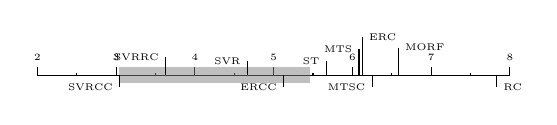
\begin{tikzpicture}
 %axis
 \draw (2,0) -- (8,0);
 \foreach \x in {2,3,4,5,6,7,8} {
  \draw (\x, 0) -- ++(0,.1) node [above,scale=0.7] {\tiny \x};
  \ifthenelse{\x < 8}{\draw (\x+.5, 0) -- ++(0,.03);}{}
 }
 % coordinates
 \coordinate (c0) at (3.0417,0);
 \coordinate (c1) at (3.6250,0);
 \coordinate (c2) at (4.6667,0);
 \coordinate (c3) at (5.1250,0);
 \coordinate (c4) at (6.1250,0);
 \coordinate (c5) at (7.8333,0);
 \coordinate (c6) at (6.2500,0);
 \coordinate (c7) at (6.0833,0);
 \coordinate (c8) at (5.6667,0);
 \coordinate (c9) at (6.5833,0);

 % labels
 \node (l0) at (c0) [below left=.025cm and 0cm, align=right,scale=0.7] {\tiny SVRCC};
 \node (l1) at (c1) [above left=.1cm and 0cm, align=right,scale=0.7] {\tiny SVRRC};
 \node (l2) at (c2) [above left=.05cm and 0cm, align=right,scale=0.7] {\tiny SVR};
 \node (l3) at (c3) [below left=.025cm and 0cm, align=left,scale=0.7] {\tiny ERCC};
 \node (l4) at (c4) [above right=.35cm and 0cm, align=right,scale=0.7] {\tiny ERC};
 \node (l5) at (c5) [below right=.025cm and 0cm, align=left,scale=0.7] {\tiny RC};
 \node (l6) at (c6) [below left=.025cm and 0cm, align=right,scale=0.7] {\tiny MTSC};
 \node (l7) at (c7) [above left=.2cm and 0cm, align=left,scale=0.7] {\tiny MTS};
 \node (l8) at (c8) [above left=.05cm and 0cm, align=right,scale=0.7] {\tiny ST};
 \node (l9) at (c9) [above right=.22cm and 0cm, align=right,scale=0.7] {\tiny MORF};

 % CD = 1.4845
 \fill[fill=gray,fill opacity=0.5] (3.0417,-0.1) rectangle (5.4653,0.1);
 
 % connectors
 \foreach \x in {0,...,9} {
  \draw (l\x) -| (c\x);
 };
\end{tikzpicture}}
\caption{\hl{Bonferroni-Dunn test for MSE}}
\label{fig:BonfDunnMSE}
\end{figure}
\vspace{-5em}
\begin{table}[H]
\centering
\caption{\hl{Wilcoxon, Nemenyi, and Holm tests for MSE}}\label{tab:statmse}
\scriptsize
\begin{threeparttable}
\begin{tabularx}{0.6\textwidth}{p{1cm}p{1cm}p{1cm}p{1cm}p{1cm}p{0.9cm}}
\toprule
SVRCC vs. & Wilcoxon $R^{+}$ & Wilcoxon $R^{-}$ & Wilcoxon $p$-value & Nemenyi $p$-value & Holm $p$-value \\
\midrule 
MORF & 268.0 & 32.0 & $3.2E^{-4}$ & $5.1E^{-5}$ & $6.3E^{-3}$ \\
ST & 241.0 & 59.0 & $7.9E^{-3}$ & $2.7E^{-3}$ & $1.3E^{-2}$ \\
MTS & 224.0 & 76.0 & $3.4E^{-2}$ & $5.0E^{-4}$ & $1.0E^{-2}$ \\
MTSC & 226.0 & 74.0 & $2.9E^{-2}$ & $2.4E^{-4}$ & $7.1E^{-3}$ \\ 
RC & 263.0 & 37.0 & $6.5E^{-4}$ & 0.0000 & $5.6E^{-3}$ \\  
ERC & 234.0 & 66.0 & $1.5E^{-2}$ & $4.2E^{-4}$ & $8.3E^{-3}$ \\
ERCC & 224.0 & 76.0 & $3.4E^{-2}$ & $1.7E^{-2}$ & $1.7E^{-2}$ \\
SVR & 262.0 & 38.0 & $7.4E^{-4}$ & $6.3E^{-2}$ & $2.5E^{-2}$ \\ 
SVRRC & 245.0 & 55.0 & $5.3E^{-3}$ & $5.1E^{-1}$ & $5.0E^{-2}$\\ 
\bottomrule 
\end{tabularx}
\begin{tablenotes}
\item Post Hoc (Friedman) comparison for $\alpha = 0.05$
\end{tablenotes}
\end{threeparttable}
\end{table}}

\subsection{Average Root Mean Square Error}\label{subsec:armse}
\hl{Table~{\ref{tab:armseresults}} shows that our proposed methods perform the best on $18$ out of the $24$ datasets. In this case, SVRCC performs the best on $15$ versus the $6$ that the state-of-the-art methods performed better at. The Iman-Davenport statistic is $7.6$, with a $p$-value of $1.3E^{-9}$, implying statistically significant differences in the aRMSE results.}

\hl{Figure~{\ref{fig:BonfDunnaRMSE}} shows the mean rank values of each algorithm along with the critical difference value, $2.4236$, for $\alpha = 0.05$. According to the critical difference bar, there are $7$ out of $10$ algorithms that perform significantly worse than our control algorithm, SVRCC.}

\hl{According to the Wilcoxon test, shown in Table~{\ref{tab:statarmse}}, SVRCC is shown to have significantly better performance over all algorithms with $p$-value $< 0.01$. The Nemenyi test shows that SVRCC performs significantly better than $7$ out of the $9$ algorithms with $p$-value $\leq 5.6E^{-3}$, while the stricter Holm test shows that it performs significantly better than $8$ out of the $9$ algorithms with $p$-value $\leq 0.05$.}

\afterpage{%
\begin{table*}[th!]
\renewcommand{\arraystretch}{1.2}
\centering
\caption{\hl{Average Root Mean Square Error (aRMSE) Results \& Algorithm Rank}}
\small
\begin{threeparttable}
\resizebox{0.9\textwidth}{!}{\begin{tabular}{lccccccccccc}
\toprule
Datasets &MORF &ST &MTS &MTSC &RC &ERC &ERCC &SVR &SVRRC &SVRCC \\
\midrule
Slump &0.6711 &0.6652 &0.6456 &0.6699 &0.6787 &0.6793 &0.6649 &0.5561 &0.5345 &\textbf{0.5337} &  \\
Polymer &0.5277 &0.5409 &0.5042 &0.5336 &0.5536 &0.5803 &0.5319 &0.4403 &0.4062 &\textbf{0.4060} &  \\
Andro &0.4649 &0.5420 &0.4414 &0.4871 &0.5390 &0.5317 &0.5039 &0.4326 &0.4061 &\textbf{0.3989} &  \\
EDM &0.6372 &0.6715 &0.6705 &0.6729 &0.6722 &0.6704 &0.6721 &0.6449 &0.6411 &\textbf{0.6366} &  \\
Solar Flare 1 &0.9777 &0.9274 &0.9271 &0.9089 &0.8921 &0.9016 &0.9121 &0.8856 &0.8844 &\textbf{0.8801} &  \\
Jura &0.5800 &0.5686 &0.5720 &0.5706 &0.5726 &0.5712 &0.5693 &0.5794 &0.5687 &\textbf{0.5622} &  \\
Enb &0.1212 &0.1166 &0.1237 &0.1214 &0.1272 &0.1253 &0.1140 &0.0981 &0.0914 &\textbf{0.0903} &  \\
Solar Flare 2 &0.8725 &0.8420 &\textbf{0.8127} &0.8305 &0.8313 &0.8300 &0.8304 &0.8418 &0.8349 &0.8345 &  \\
Wisconsin Cancer &0.9290 &0.9163 &0.9158 &0.9187 &\textbf{0.9153} &0.9160 &0.9173 &0.9422 &0.9362 &0.9306 &  \\
California Housing &0.6541 &0.6366 &0.6889 &0.6530 &0.7053 &0.6632 &0.6079 &0.6038 &0.5859 &\textbf{0.5755} &  \\
Stock &0.1643 &0.1830 &0.1774 &0.1790 &0.1790 &0.1777 &0.1739 &0.1357 &0.1329 &\textbf{0.1308} &  \\
SCPF &0.7113 &0.7235 &0.7342 &0.7255 &0.7285 &0.7143 &0.7227 &0.7155 &0.7081 &\textbf{0.7048} &  \\
Puma8NH &0.7855 &0.8139 &0.8114 &0.8307 &0.8196 &0.8202 &0.8203 &\textbf{0.7650} &0.7740 &0.7671 &  \\
Friedman &0.9382 &0.9203 &0.9219 &0.9199 &0.9219 &0.9197 &0.9193 &0.9203 &0.9195 &\textbf{0.9183} &  \\
Puma32H &0.9395 &\textbf{0.8700} &0.8713 &0.8778 &0.8739 &0.8716 &0.8727 &0.9353 &0.9356 &0.9331 &  \\
Water Quality &\textbf{0.8921} &0.9015 &0.9041 &0.9025 &0.9051 &0.9030 &0.8990 &0.9284 &0.9293 &0.9271 &  \\
M5SPEC &0.5707 &0.5324 &0.5761 &0.5515 &0.5347 &0.5339 &0.5376 &0.2745 &0.2744 &\textbf{0.2740} &  \\
MP5SPEC &0.5315 &0.4914 &0.5426 &0.4947 &0.4930 &0.4928 &0.4928 &0.2337 &\textbf{0.2176} &0.2177 &  \\
MP6SPEC &0.5344 &0.4939 &0.5416 &0.4943 &0.4982 &0.4967 &0.4927 &0.2627 &\textbf{0.2460} &0.2497 &  \\
ATP7d &0.5216 &0.4956 &\textbf{0.4752} &0.4765 &0.5194 &0.5024 &0.4824 &0.5141 &0.5066 &0.5018 &  \\
OES97 &0.4652 &0.4634 &0.4635 &0.4622 &0.4643 &0.4644 &0.4627 &0.3794 &0.3768 &\textbf{0.3749} &  \\
Osales &0.7190 &0.6912 &\textbf{0.6496} &0.6615 &0.7591 &0.6772 &0.6515 &0.7212 &0.7343 &0.7121 &  \\
ATP1d &0.4053 &0.3608 &0.3587 &0.3591 &0.3653 &0.3562 &0.3596 &0.3693 &0.3638 &\textbf{0.3507} &  \\
OES10 &0.3954 &0.3896 &0.3897 &0.3892 &0.3901 &0.3903 &0.3889 &0.3085 &0.3039 &\textbf{0.3038} &  \\
\hline
Average &0.6254 &0.6149 &0.6133 &0.6121 &0.6225 &0.6162 &0.6083 &0.5620 &0.5547 &\textbf{0.5506} &  \\
Ranks &7.3333 &5.7708 &5.8125 &6.0625 &7.6250 &6.0208 &4.8542 &5.0625 &3.9167 &\textbf{2.5417} &  \\
\bottomrule
\end{tabular}}
\end{threeparttable}
\label{tab:armseresults}
\end{table*}
\vspace{-1.7em}
\begin{figure}[h!]
\centering
\small
\resizebox{0.8\textwidth}{!}{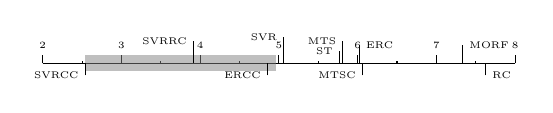
\begin{tikzpicture}
 %axis
 \draw (2,0) -- (8,0);
 \foreach \x in {2,3,4,5,6,7,8} {
  \draw (\x, 0) -- ++(0,.1) node [above,scale=0.7] {\tiny \x};
  \ifthenelse{\x < 8}{\draw (\x+.5, 0) -- ++(0,.03);}{}
 }
 % coordinates
 \coordinate (c0) at (2.5417,0);
 \coordinate (c1) at (3.9167,0);
 \coordinate (c2) at (5.0625,0);
 \coordinate (c3) at (4.8542,0);
 \coordinate (c4) at (6.0208,0);
 \coordinate (c5) at (7.6250,0);
 \coordinate (c6) at (6.0625,0);
 \coordinate (c7) at (5.8125,0);
 \coordinate (c8) at (5.7708,0);
 \coordinate (c9) at (7.3333,0);

 % labels
 \node (l0) at (c0) [below left=.025cm and 0cm, align=right,scale=0.7] {\tiny SVRCC};
 \node (l1) at (c1) [above left=.15cm and 0cm, align=right,scale=0.7] {\tiny SVRRC};
 \node (l2) at (c2) [above left=.2cm and 0cm, align=right,scale=0.7] {\tiny SVR};
 \node (l3) at (c3) [below left=.025cm and 0cm, align=left,scale=0.7] {\tiny ERCC};
 \node (l4) at (c4) [above right=.1cm and 0cm, align=right,scale=0.7] {\tiny ERC};
 \node (l5) at (c5) [below right=.025cm and 0cm, align=left,scale=0.7] {\tiny RC};
 \node (l6) at (c6) [below left=.025cm and 0cm, align=right,scale=0.7] {\tiny MTSC};
 \node (l7) at (c7) [above left=.15cm and 0cm, align=left,scale=0.7] {\tiny MTS};
 \node (l8) at (c8) [above left=.025cm and 0cm, align=right,scale=0.7] {\tiny ST};
 \node (l9) at (c9) [above right=.1cm and 0cm, align=right,scale=0.7] {\tiny MORF};

 % CD = 1.4845
 \fill[fill=gray,fill opacity=0.5] (2.5417,-0.1) rectangle (4.9653,0.1);
 
 % connectors
 \foreach \x in {0,...,9} {
  \draw (l\x) -| (c\x);
 };
\end{tikzpicture}}
\caption{\hl{Bonferroni-Dunn test for aRMSE}}
\label{fig:BonfDunnaRMSE}
\end{figure}
\vspace{-1.7em}
\begin{table}[H]
\centering
\caption{\hl{Wilcoxon, Nemenyi, and Holm tests for aRMSE}}\label{tab:statarmse}
\scriptsize
\begin{threeparttable}
\begin{tabularx}{0.6\textwidth}{p{1cm}p{1cm}p{1cm}p{1cm}p{1cm}p{0.9cm}}
SVRCC vs. & Wilcoxon $R^{+}$ & Wilcoxon $R^{-}$ & Wilcoxon $p$-value & Nemenyi $p$-value & Holm $p$-value \\ \hline 
MORF & 286.0 & 14.0 & $1.3E^{-5}$ & 0.0000 & $6.3E^{-3}$ \\
ST & 259.0 & 41.0 & $1.1E^{-3}$ & $2.2E^{-4}$ & $1.3E^{-2}$ \\
MTS & 247.0 & 53.0 & $4.3E^{-3}$ & $1.8E^{-5}$ & $1.0E^{-2}$ \\ 
MTSC & 251.0 & 49.0 & $2.8E^{-3}$ & $5.6E^{-5}$ & $7.1E^{-3}$ \\
RC & 270.0 & 30.0 & $2.4E^{-4}$ & 0.0000 & $5.6E^{-3}$ \\ 
ERC & 255.0 & 45.0 & $1.8E^{-3}$ & $6.9E^{-5}$ & $8.3E^{-3}$ \\
ERCC & 246.0 & 54.0 & $4.8E^{-3}$ & $8.2E^{-3}$ & $2.5E^{-2}$ \\
SVR & 296.0 & 4.00 & $8.3E^{-7}$ & $3.9E^{-3}$ & $1.7E^{-2}$ \\
SVRRC & 284.0 & 16.0 & $2.0E^{-5}$ & $1.2E^{-1}$ & $5.0E^{-2}$ \\  \hline 
\end{tabularx}
\begin{tablenotes}
\item Post Hoc (Friedman) comparison for $\alpha = 0.05$
\end{tablenotes}
\end{threeparttable}
\end{table}}

\subsection{Average Relative Root Mean Square Error}\label{subsec:arrmse}
\hl{Table~{\ref{tab:arrmseresults}} shows that our proposed methods perform the best on $16$ out of the $24$ datasets. In this case, SVRCC performs the best on $11$ versus the $6$ that the state-of-the-art methods performed better at. The Iman-Davenport statistic is $8.54$, with a $p$-value of $7.6E^{-11}$.}

\hl{Figure~{\ref{fig:BonfDunnaRRMSE}} shows the mean rank values of each algorithm along with the critical difference value, $2.4236$, for $\alpha = 0.05$. According to the critical difference bar, there are $6$ out of $10$ algorithms beyond that perform significantly worse than our control algorithm, SVRCC.}

\hl{According to the Wilcoxon test, shown in Table~{\ref{tab:statarrmse}}, SVRCC is shown to have significantly better performance over all algorithms with $p$-value $< 0.05$, and $8$ out of the $9$ algorithms for $p$-value $< 0.01$. The Nemenyi test shows that SVRCC performs significantly better than $6$ out of the $9$ algorithms with $p$-value $\leq 5.6E^{-3}$, and the Holm test shows its performance is significantly better than $8$ out of the $9$ algorithms with $p$-value $\leq 0.05$.}

\afterpage{%
\begin{table*}[t!]
\renewcommand{\arraystretch}{1.2}
\centering
\caption{\hl{Average Relative Root Mean Square Error (aRRMSE) Results \& Algorithm Rank}}
\begin{threeparttable}
\resizebox{0.9\textwidth}{!}{\begin{tabular}{lccccccccccc}
\toprule
Datasets &MORF &ST &MTS &MTSC &RC &ERC &ERCC &SVR &SVRRC &SVRCC \\
\midrule
Slump &0.6939 &0.6886 &0.6690 &0.6938 &0.7019 &0.7022 &0.6886 &0.5765 &\textbf{0.5545} &0.5560 &  \\
Polymer &0.6159 &0.5971 &0.5778 &0.6493 &0.6270 &0.6544 &0.6131 &0.5573 &0.5253 &\textbf{0.5116} &  \\
Andro &0.5097 &0.5979 &0.5155 &0.5633 &0.5924 &0.5885 &0.5666 &0.4856 &0.4651 &\textbf{0.4455} &  \\
EDM &0.7337 &0.7442 &0.7413 &0.7446 &0.7449 &0.7452 &0.7443 &0.7058 &0.7070 &\textbf{0.6978} &  \\
Solar Flare 1 &1.3046 &1.1357 &1.1168 &1.0758 &0.9951 &1.0457 &1.0887 &0.9917 &0.9455 &\textbf{0.9320} &  \\
Jura &0.5969 &0.5874 &0.5906 &0.5892 &0.5910 &0.5896 &0.5880 &0.5952 &\textbf{0.5764} &0.5885 &  \\
Enb &0.1210 &0.1165 &0.1231 &0.1211 &0.1268 &0.1250 &0.1139 &0.0977 &0.0910 &\textbf{0.0899} &  \\
Solar Flare 2 &1.4167 &1.1503 &\textbf{0.9483} &1.0840 &1.0092 &1.0522 &1.0928 &1.0385 &1.0253 &1.0298 &  \\
Wisconsin Cancer &0.9413 &0.9314 &0.9308 &0.9336 &\textbf{0.9305} &0.9313 &0.9323 &0.9555 &0.9483 &0.9427 &  \\
California Housing &0.6611 &0.6447 &0.6974 &0.6630 &0.7131 &0.6690 &0.6146 &0.6130 &0.5945 &\textbf{0.5852} &  \\
Stock &0.1653 &0.1844 &0.1787 &0.1803 &0.1802 &0.1789 &0.1752 &0.1364 &\textbf{0.1337} &0.1388 &  \\
SCPF &0.8273 &0.8348 &0.8436 &0.8308 &0.8263 &0.8105 &0.8290 &0.8164 &0.8037 &\textbf{0.8013} &  \\
Puma8NH &0.7858 &0.8142 &0.8118 &0.8311 &0.8199 &0.8205 &0.8207 &\textbf{0.7655} &0.7744 &0.7676 &  \\
Friedman &0.9394 &0.9214 &0.9231 &0.9210 &0.9231 &0.9209 &0.9204 &0.9218 &0.9208 &\textbf{0.9196} &  \\
Puma32H &0.9406 &\textbf{0.8713} &0.8727 &0.8791 &0.8752 &0.8729 &0.8740 &0.9364 &0.9367 &0.9319 &  \\
Water Quality &\textbf{0.8994} &0.9085 &0.9109 &0.9093 &0.9121 &0.9097 &0.9057 &0.9343 &0.9310 &0.9045 &  \\
M5SPEC &0.5910 &0.5523 &0.5974 &0.5671 &0.5552 &0.5542 &0.5558 &0.2951 &0.2935 &\textbf{0.2925} &  \\
MP5SPEC &0.5522 &0.5120 &0.5683 &0.5133 &0.5145 &0.5143 &0.5119 &0.2484 &\textbf{0.2323} &0.2358 &  \\
MP6SPEC &0.5553 &0.5152 &0.5686 &0.5119 &0.5198 &0.5187 &0.5109 &0.2850 &0.2669 &\textbf{0.2623} &  \\
ATP7d &0.5563 &0.5308 &\textbf{0.5141} &0.5142 &0.5558 &0.5397 &0.5182 &0.5455 &0.5371 &0.5342 &  \\
OES97 &0.5490 &0.5230 &0.5229 &0.5217 &0.5239 &0.5237 &0.5222 &0.4641 &\textbf{0.4618} &0.4635 &  \\
Osales &0.7596 &0.7471 &\textbf{0.7086} &0.7268 &0.8318 &0.7258 &0.7101 &0.7924 &0.7924 &0.7811 &  \\
ATP1d &0.4173 &0.3732 &0.3733 &0.3712 &0.3790 &\textbf{0.3696} &0.3721 &0.3773 &0.3707 &0.3775 &  \\
OES10 &0.4518 &0.4174 &0.4176 &0.4171 &0.4178 &0.4180 &0.4166 &0.3570 &0.3555 &\textbf{0.3538} &  \\
\hline
Average &0.6910 &0.6625 &0.6551 &0.6589 &0.6611 &0.6575 &0.6536 &0.6039 &0.5935 &\textbf{0.5893} &  \\
Ranks &7.5000 &5.7708 &5.9375 &6.1667 &7.4375 &6.3750 &4.9792 &4.7708 &3.2708 &\textbf{2.7917} &  \\
\bottomrule
\end{tabular}}
\end{threeparttable}
\label{tab:arrmseresults}
\end{table*}
\vspace{-2.7em}
\begin{figure}[h!]
\centering
\small
\resizebox{0.8\textwidth}{!}{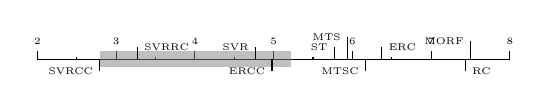
\begin{tikzpicture}
 %axis
 \draw (2,0) -- (8,0);
 \foreach \x in {2,3,4,5,6,7,8} {
  \draw (\x, 0) -- ++(0,.1) node [above,scale=0.7] {\tiny \x};
  \ifthenelse{\x < 8}{\draw (\x+.5, 0) -- ++(0,.03);}{}
 }
 % coordinates
 \coordinate (c0) at (2.7917,0);
 \coordinate (c1) at (3.2708,0);
 \coordinate (c2) at (4.7708,0);
 \coordinate (c3) at (4.9792,0);
 \coordinate (c4) at (6.3750,0);
 \coordinate (c5) at (7.4375,0);
 \coordinate (c6) at (6.1667,0);
 \coordinate (c7) at (5.9375,0);
 \coordinate (c8) at (5.7708,0);
 \coordinate (c9) at (7.5000,0);

 % labels
 \node (l0) at (c0) [below left=.025cm and 0cm, align=right,scale=0.7] {\tiny SVRCC};
 \node (l1) at (c1) [above right=.025cm and 0cm, align=right,scale=0.7] {\tiny SVRRC};
 \node (l2) at (c2) [above left=.025cm and 0cm, align=right,scale=0.7] {\tiny SVR};
 \node (l3) at (c3) [below left=.025cm and 0cm, align=left,scale=0.7] {\tiny ERCC};
 \node (l4) at (c4) [above right=.025cm and 0cm, align=right,scale=0.7] {\tiny ERC};
 \node (l5) at (c5) [below right=.025cm and 0cm, align=left,scale=0.7] {\tiny RC};
 \node (l6) at (c6) [below left=.025cm and 0cm, align=right,scale=0.7] {\tiny MTSC};
 \node (l7) at (c7) [above left=.15cm and 0cm, align=left,scale=0.7] {\tiny MTS};
 \node (l8) at (c8) [above left=.025cm and 0cm, align=right,scale=0.7] {\tiny ST};
 \node (l9) at (c9) [above left=.1cm and 0cm, align=right,scale=0.7] {\tiny MORF};

 % CD = 1.4845
 \fill[fill=gray,fill opacity=0.5] (2.7917,-0.1) rectangle (5.2153,0.1);
 
 % connectors
 \foreach \x in {0,...,9} {
  \draw (l\x) -| (c\x);
 };
\end{tikzpicture}}
\caption{\hl{Bonferroni-Dunn test for aRRMSE}}
\label{fig:BonfDunnaRRMSE}
\end{figure}
\vspace{-2em}
\begin{table}[H]
\centering
\caption{\hl{Wilcoxon, Nemenyi, and Holm tests for aRRMSE}}\label{tab:statarrmse}
\scriptsize
\begin{threeparttable}
\begin{tabularx}{0.6\textwidth}{p{1cm}p{1cm}p{1cm}p{1cm}p{1cm}p{0.9cm}}
\toprule
SVRCC vs. & Wilcoxon $R^{+}$ & Wilcoxon $R^{-}$ & Wilcoxon $p$-value & Nemenyi $p$-value & Holm $p$-value \\ 
\midrule 
MORF & 290.0 & 10.0 & $5.1E^{-6}$ & $0.0000$ & $5.6E^{-3}$ \\  
ST & 261.0 & 39.0 & $8.5E^{-4}$ & $6.5E^{-4}$ & $1.3E^{-2}$\\
MTS & 239.0 & 61.0 & $9.6E^{-3}$ & $3.2E^{-3}$ & $1.0E^{-2}$\\ 
MTSC & 261.0 & 39.0 & $8.5E^{-4}$ & $1.1E^{-3}$ & $8.3E^{-3}$\\  
RC & 275.0 & 25.0 & $1.1E^{-4}$ & 0.0000 & $6.3E^{-3}$ \\
ERC & 261.0 & 39.0 & $8.5E^{-4}$ & $4.1E^{-5}$ & $7.1E^{-3}$\\ 
ERCC & 254.0 & 46.0 & $2.0E^{-3}$ & $1.2E^{-2}$ & $1.7E^{-2}$\\
SVR & 291.0 & 9.00 & $3.9E^{-6}$ & $2.4E^{-2}$ & $2.5E^{-2}$\\
SVRRC & 222.5 & 77.5 & $3.8E^{-2}$ & $5.8E^{-1}$ & $5.0E^{-2}$ \\ 
\bottomrule 
\end{tabularx}
\begin{tablenotes}
\item Post Hoc (Friedman) comparison for $\alpha = 0.05$
\end{tablenotes}
\end{threeparttable}
\end{table}}

\newpage
\subsection{Run Time}\label{subsec:time}
\hl{Table~{\ref{tab:timeresults}} shows that our proposed methods perform faster on $16$ out of the $24$ datasets. In this case, SVR performs the best on $12$ versus the $6$ of the state-of-the-art methods. The Iman-Davenport statistic $64.41$, with a $p$-value of $0.0$ which implies a statistical confidence of $100\%$.}

\hl{Figure~{\ref{fig:BonfDunnTime}} shows the mean rank values of each algorithm along with the critical difference value, $2.4236$, for $\alpha = 0.05$. According to the critical difference bar, there are $6$ out of $10$ algorithms beyond that perform significantly worse than our control algorithm, SVR.}
\hl{According to the Wilcoxon test, shown in Table~{\ref{tab:stattime}}, SVR is shown to have significantly better performance over all algorithms with $p$-value $< 0.01$. The Nemenyi and Holm tests show that SVRCC performs significantly better than $6$ out of the $9$ algorithms and $8$ out of the $9$ algorithms with $p$-value $\leq 5.6E^{-3}$ and $p$-value $\leq 1.6E^{-2}$, respectively.}

\afterpage{%
\begin{table*}[th!]
\renewcommand{\arraystretch}{1.2}
\centering
\caption{\hl{Run Time Results (s) \& Algorithm Rank}}
\small
\resizebox{0.9\textwidth}{!}{\begin{threeparttable}
\resizebox{\textwidth}{!}{\begin{tabular}{lccccccccccc}
\toprule
Datasets &MORF &ST &MTS &MTSC &RC &ERC &ERCC &SVR &SVRRC &SVRCC \\
\midrule
Slump &38.1 &2.6 &9.9 &15.9 &1.8 &11.1 &50.5 &\textbf{0.6} &1.9 &0.7 &  \\
Polymer &7.6 &2.7 &9.1 &15.5 &1.9 &14.9 &80.5 &\textbf{0.5} &2.6 &\textbf{0.5} &  \\
Andro &25.7 &4.4 &15.0 &34.2 &3.4 &33.2 &197.9 &\textbf{1.1} &6.2 &\textbf{1.1} &  \\
EDM &24.8 &2.8 &9.4 &18.1 &2.1 &5.8 &19.0 &\textbf{0.9} &1.0 &\textbf{0.9} &  \\
Solar Flare 1 &34.1 &3.5 &13.6 &26.7 &2.7 &17.7 &86.9 &\textbf{2.3} &9.3 &2.6 &  \\
Jura &64.3 &7.9 &31.8 &74.3 &6.4 &43.5 &254.2 &\textbf{4.7} &18.7 &5.3 &  \\
Enb &71.4 &6.6 &26.1 &63.6 &\textbf{5.4} &15.6 &69.6 &11.3 &17.7 &15.9 &  \\
Solar Flare 2 &55.4 &7.4 &30.7 &68.0 &\textbf{6.3} &42.9 &241.5 &9.4 &53.5 &15.6 &  \\
Wisconsin Cancer &51.4 &6.1 &21.9 &53.7 &4.9 &14.8 &61.6 &\textbf{2.0} &2.4 &\textbf{2.0} &  \\
California Housing &93.0 &9.7 &34.8 &75.9 &\textbf{8.2} &21.3 &102.0 &15.8 &25.2 &23.6 &  \\
Stock &93.7 &11.7 &46.8 &96.7 &\textbf{11.0} &75.4 &427.3 &18.5 &90.5 &26.3 &  \\
SCPF &66.3 &19.3 &65.9 &176.3 &\textbf{15.0} &104.2 &734.2 &32.8 &162.8 &48.8 &  \\
Puma8NH &130.4 &29.7 &106.7 &288.6 &\textbf{27.9} &201.6 &1227.7 &94.1 &516.6 &177.1 &  \\
Friedman &79.5 &27.0 &81.2 &258.3 &25.0 &273.7 &2871.6 &\textbf{12.3} &322.3 &18.8 &  \\
Puma32H &93.9 &68.1 &181.0 &635.0 &87.7 &667.9 &6087.0 &\textbf{32.2} &1018.7 &53.1 &  \\
Water Quality &108.4 &\textbf{93.1} &262.1 &912.3 &127.2 &925.4 &10993.3 &110.2 &2567.9 &189.5 &  \\
M5SPEC &89.8 &68.9 &166.3 &604.6 &73.7 &262.3 &3132.1 &\textbf{39.2} &546.7 &45.1 &  \\
MP5SPEC &84.5 &94.6 &221.2 &888.3 &91.5 &557.0 &6864.1 &\textbf{49.3} &1132.1 &58.4 &  \\
MP6SPEC &90.3 &93.4 &212.6 &871.0 &89.1 &557.6 &6761.3 &\textbf{47.2} &1227.1 &58.5 &  \\
ATP7d &\textbf{70.5} &262.6 &452.1 &2319.8 &242.1 &1779.2 &24373.8 &80.0 &1897.4 &136.5 &  \\
OES97 &\textbf{83.4} &485.3 &1146.6 &4928.9 &499.8 &5315.0 &58072.1 &148.2 &3759.1 &342.6 &  \\
Osales &\textbf{92.0} &1094.8 &2340.7 &8322.2 &986.5 &11361.2 &122265.3 &437.0 &4830.1 &843.6 &  \\
ATP1d &\textbf{70.7} &272.9 &476.5 &2568.9 &261.9 &2138.9 &26768.9 &95.0 &2127.8 &174.4 &  \\
OES10 &\textbf{90.0} &738.9 &1633.6 &6682.9 &688.5 &7150.8 &83533.1 &229.1 &5419.4 &577.1 &  \\
\hline
Average &71.2 &142.2 &316.5 &1250.0 &136.2 &1316.3 &14803.2 &\textbf{61.4} &1073.2 &117.4 &  \\
Ranks &5.5 &3.71 &6.0 &8.29 &3.0 &7.08 &9.92 &\textbf{1.88} &6.71 &2.92 &  \\
\bottomrule
\end{tabular}}
\end{threeparttable}}
\label{tab:timeresults}
\end{table*}
\vspace{-1.6em}
\begin{figure}[h!]
\centering
\resizebox{\textwidth}{!}{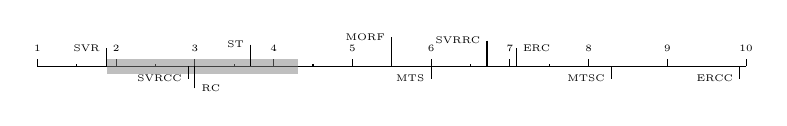
\begin{tikzpicture}
 %axis
 \draw (1,0) -- (10,0);
 \foreach \x in {1,2,3,4,5,6,7,8,9,10} {
  \draw (\x, 0) -- ++(0,.1) node [above,scale=0.7] {\tiny \x};
  \ifthenelse{\x < 8}{\draw (\x+.5, 0) -- ++(0,.03);}{}
 }
 % coordinates
 \coordinate (c0) at (2.92,0);
 \coordinate (c1) at (6.71,0);
 \coordinate (c2) at (1.88,0);
 \coordinate (c3) at (9.92,0);
 \coordinate (c4) at (7.08,0);
 \coordinate (c5) at (3,0);
 \coordinate (c6) at (8.29,0);
 \coordinate (c7) at (6,0);
 \coordinate (c8) at (3.71,0);
 \coordinate (c9) at (5.5,0);

 % labels
 \node (l0) at (c0) [below left=.025cm and 0cm, align=right,scale=0.7] {\tiny SVRCC};
 \node (l1) at (c1) [above left=.2cm and 0cm, align=right,scale=0.7] {\tiny SVRRC};
 \node (l2) at (c2) [above left=.1cm and 0cm, align=right,scale=0.7] {\tiny SVR};
 \node (l3) at (c3) [below left=.025cm and 0cm, align=left,scale=0.7] {\tiny ERCC};
 \node (l4) at (c4) [above right=.1cm and 0cm, align=right,scale=0.7] {\tiny ERC};
 \node (l5) at (c5) [below right=.15cm and 0cm, align=left,scale=0.7] {\tiny RC};
 \node (l6) at (c6) [below left=.025cm and 0cm, align=right,scale=0.7] {\tiny MTSC};
 \node (l7) at (c7) [below left=.025cm and 0cm, align=left,scale=0.7] {\tiny MTS};
 \node (l8) at (c8) [above left=.15cm and 0cm, align=right,scale=0.7] {\tiny ST};
 \node (l9) at (c9) [above left=.24cm and 0cm, align=right,scale=0.7] {\tiny MORF};

 % CD = 1.4845
 \fill[fill=gray,fill opacity=0.5] (1.88,-0.1) rectangle (4.3036,0.1);
 
 % connectors
 \foreach \x in {0,...,9} {
  \draw (l\x) -| (c\x);
 };
\end{tikzpicture}}
\caption{\hl{Bonferroni-Dunn test for Run Time}}
\label{fig:BonfDunnTime}
\end{figure}
\vspace{-1.7em}
\begin{table}[H]
\centering
\caption{\hl{Wilcoxon, Nemenyi, and Holm tests for Run Time}}\label{tab:stattime}
\scriptsize
\begin{threeparttable}
\begin{tabularx}{0.6\textwidth}{p{1cm}p{1cm}p{1cm}p{1cm}p{1cm}p{0.9cm}}
\toprule
SVR vs. & Wilcoxon $R^{+}$ & Wilcoxon $R^{-}$ & Wilcoxon $p$-value & Nemenyi $p$-value & Holm $p$-value \\ 
\midrule 
SVRCC & 295.0 & 5.00 & $1.2E^{-6}$ &  $2.3E^{-1}$ & $5.0E^{-2}$\\ 
MORF & 225.0 & 75.0 & $3.2E^{-2}$ &  $3.4E^{-5}$ & $1.3E^{-2}$\\  
ST & 221.5 & 78.5 & $4.1E^{-2}$ &  $3.6E^{-2}$ & $1.7E^{-2}$\\   
MTS & 300.0 & 0.00 & $1.2E^{-7}$ &  $2.0E^{-6}$ & $1.0E^{-2}$\\ 
MTSC & 300.0 & 0.00 & $1.2E^{-7}$ &  0.0000 & $6.3E^{-3}$\\
RC & 229.0 & 71.0 & $2.3E^{-2}$ &  $2.0E^{-1}$ & $2.5E^{-2}$ \\  
ERC & 300.0 & 0.00 & $1.2E^{-7}$ & 0.0000 & $7.1E^{-3}$\\  
ERCC & 300.0 & 0.00 & $1.2E^{-7}$ & 0.0000 & $5.6E^{-3}$\\ 
SVRRC & 300.0 & 0.00 & $1.2E^{-7}$ &  0.0000 & $8.3E^{-3}$\\ 
\bottomrule
\end{tabularx}
\begin{tablenotes}
\item Post Hoc (Friedman) comparison for $\alpha = 0.05$
\end{tablenotes}
\end{threeparttable}
\end{table}}

\subsection{Discussion}\label{sec:discussion}
\hl{Results indicate that our proposed methods perform competitively against the current state-of-the-art, specifically SVRCC which exploits relationships among the targets. Firstly, they show that using SVR as a base-line method for multi-target chaining causes a performance improvement in model prediction, compared to other ST base-line models, as well as most MT methods. This demonstrates the advantages of using the SVR method as a base-line for multi-target learning, thus increasing the performance of the ensemble of regressor chains, SVRRC, compared to the state-of-the-art ERCC. More importantly, the results highlight the major advantage of capturing and exploiting the targets' relationships during model training. Using an ensemble of randomly generated chains does not ensure the targets' correlations are fully captured; however, using a maximum correlation chain improves the performance in terms of quality metrics as well as run time. The run time of SVR was shown to be the fastest, due to the fact that its complexity is mostly dependent on the number of targets. However, this method does not consider any of the correlations that might exist among the target variables, but SVRCC does take them into account and does not have a significant impact on run time. The most noteworthy finding that highlights advantage of using the base-line SVR and the maximum correlation method, SVRCC, rather than random chaining as done in ERCC, are the run time results and their analysis. ERCC had the worst run time across all datasets, whereas our proposals, SVR and SVRCC, performed the fastest. This emphasizes the advantage of using a single chain rather an ensemble of random chains, especially when the single chain is ordered in the direction of the targets maximum correlation.}

\section{Conclusion}\label{sec:conclusions}
This paper proposed three novel methods for solving multi-target regression problems. The first method takes a \textit{problem transformation} approach, which generates $m$ \hl{ST models, each trained independently.} This \hl{base-line} approach \hl{was shown to perform the best in terms of run time, but its drawback  is that it does not take the possible correlations between the target variables into account during training. The second implements SVR as an ensemble model of randomly generated chains, inspired by the state-of-the-art classification method ERCC. This was done to investigate the effects of exploiting correlations among the target variables during model training. Due to the random nature of this method, capturing target correlations is not guaranteed. The third proposal, SVRCC, generates a single chain that is ordered in the direction of the targets' maximum correlation, ensuring the correlations among targets are taken into account within the learning process.}

\hl{The experimental study compared the proposed methods' performances to $7$ state-of-the-art methods on 24 MT regression datasets. Firstly, the results show the superior performance of using the SVR method as a base-line model, rather than regression trees as used in MORF. The results for SVRRC show an increase in performance when random chaining is used to develop an ensemble model. This indicates} the importance of the relationship among the target variables \hl{during} training. Finally, the results show the superiority of using the SVRCC method, which \hl{was ranked the best in all quality metrics and second best in terms of run time. SVRCC performed better than the single-target SVR model and the randomly chained ensemble model SVRRC, showing that the targets' maximum correlation does positively contribute toward model training.} The statistical analysis supports and shows the significance of the results obtained by our experiments. They demonstrated that statistically significant differences exist between \hl{the proposed algorithms against the state-of-the-art methods. SVRCCs competitive performance, as well as speed, shows} that it is a powerful learning algorithm for multi-target problems. 

% regular IEEE prefers the singular form
\section*{Acknowledgment}

This research was supported by the Spanish Ministry of Economy and Competitiveness, project TIN2014-55252-P, and by FEDER funds.

\bibliographystyle{model1-num-names}
\bibliography{references}

\end{document}